\documentclass[brazil,12p,A4,openany,normaltoc,pnumromarab]{abnt}
\usepackage{paralist}
\usepackage{graphicx,url,subfigure}
\usepackage[brazil]{babel}
\usepackage[utf8]{inputenc}
\usepackage[T1]{fontenc}
\usepackage{ae}
\usepackage[alf,bibjustif,abnt-etal-list=0]{abntcite}
\usepackage{alltt}
\usepackage{booktabs}
\usepackage{nomencl}
\usepackage{amssymb}
\usepackage{amsmath}
\usepackage[left=3cm,top=3cm,right=2cm,bottom=2cm]{geometry}
\usepackage[nice]{nicefrac}

\usepackage{rotating}
\usepackage{multirow}

\usepackage{color}
\usepackage{caption}
\usepackage{listings}
\lstset{
  basicstyle=\footnotesize\ttfamily,
  stepnumber=1,
  numbersep=5pt,
  tabsize=2,
  extendedchars=true,
  breaklines=true,
  keywordstyle=\bfseries,
  showspaces=false,
  showtabs=false,
  xleftmargin=17pt,
  framexleftmargin=17pt,
  framexrightmargin=5pt,
  framexbottommargin=4pt,
  showstringspaces=false,
}
\lstloadlanguages{
  Tcl, C
}

\DeclareCaptionFont{black}{\color{black}}
\DeclareCaptionFormat{listing}{#1#2#3}
\captionsetup[lstlisting]{format=listing, textfont=black,
  }

\makeatletter

\newcommand{\up}[1]{\raisebox{1.5ex}[0pt]{#1}}
\newcommand{\doctitulo}{Tcl JIT}
\newcommand{\docautor}{Guilherme Henrique Polo Gonçalves}
\newcommand{\docorient}{Prof. Dr. Anderson Faustino da Silva}


\renewcommand{\nomname}{Lista de Siglas}
\makenomenclature

\begin{document}

\baselineskip=.7cm

\thispagestyle{empty}

\vspace{4cm}

\begin{center}

\textbf{UNIVERSIDADE ESTADUAL DE MARINGÁ}

\textbf{CENTRO DE TECNOLOGIA}

\textbf{DEPARTAMENTO DE INFORMÁTICA}

\vspace{4cm}

\textbf{\MakeUppercase{\doctitulo}}

\vspace{1cm}

\MakeUppercase{\docautor}

\vspace{1cm}

\textbf{TG-CC-10}

\end{center}

\vspace{11cm}

\begin{center}
\centering
\textbf{Maringá - Paraná}

\textbf{2010}
\end{center}


\pagebreak

\thispagestyle{empty}

\vspace{4cm}

\begin{center}

\textbf{UNIVERSIDADE ESTADUAL DE MARINGÁ}

\textbf{CENTRO DE TECNOLOGIA}

\textbf{DEPARTAMENTO DE INFORMÁTICA}

\vspace{4cm}

\textbf{\doctitulo}

\vspace{1cm}

\docautor

\vspace{1cm}

\textbf{TG-CC-10}

\end{center}

\vspace{3cm}

\begin{flushright}
\parbox{9cm}
{
\baselineskip .7cm
Trabalho de Conclusão de Curso apresentado ao Curso de Ciência da Computação,
do Centro de Tecnologia, da Universidade Estadual de Maringá.

Orientador: \docorient
}
\end{flushright}

\vspace{5cm}

\begin{center}
\centering
\textbf{Maringá - Paraná}

\textbf{2010}
\end{center}


\pagebreak

\thispagestyle{empty}
\begin{center}
\textbf{\MakeUppercase{\docautor}}

\vspace{4cm}

\textbf{\MakeUppercase{\doctitulo}}

\vspace{2cm}

Este exemplar corresponde à redação final da monografia
aprovada como requisito parcial para obtenção do grau de
Bacharel em Ciência da Computação da Universidade Estadual de
Maringá, pela Banca Examinadora formada pelos
seguintes membros:

\end{center}

\vspace{2cm}

\begin{flushright}
\parbox{10cm}
{
\begin{center}

\rule{10cm}{.02cm} \\
Prof. Dr. Anderson Faustino da Silva \\
Departamento de Informática, CTC, DIN\\
\vspace{.40in}

\rule{10cm}{.02cm} \\
Profa. Dra. Valéria Delisandra Feltrim \\
Departamento de Informática, CTC, DIN\\
\vspace{.40in}

\rule{10cm}{.02cm} \\
Prof. Ms. José Roberto Vasconcelos \\
Departamento de Informática, CTC, DIN\\

\end{center}
}
\end{flushright}

\vspace{1cm}

\begin{center}
\centering
\textbf{Maringá - Paraná}

\textbf{2010}
\end{center}


\pagebreak

\thispagestyle{empty}
\textbfsf{Resumo}\\
Linguagens de programação interpretadas tem trocado performance por
maior expressividade, flexibilidade, dinamicidade, entre outros.
Reescrita de trechos de código críticos em linguagens compiladas tem
sido empregada como meio de reduzir o impacto da máquina virtual no
tempo de execução de programas. Diante disso, um compilador JIT para a
linguagem de programação Tcl é proposto como forma de diminuir a
necessidade de tal reescrita de código. Um modo misto de execução é
escolhido, fazendo com que execução de código de máquina, gerado por
esse compilador dinâmico, e a interpretação pura se
alternem. Procedimentos são definidos como os limites de inicio e
término de compilação, e a compilação baseada em regiões é rapidamente
mencionada. Simplicidade, manutenibilidade e flexibilidade são
características que serão seguidas na construção dessa ferramenta.
Algumas conclusões iniciais a respeito de máquinas virtuais baseadas
em pilha e também sobre aquelas baseadas em registradores são feitas
de acordo com o desenvolvimento do projeto até o momento.

\quad\\
\quad\\
\textit{Palavras-chave}: Tcl, JIT, código de máquina

\thispagestyle{empty}

{
\Large
\begin{center}
\textbf{Abstract}
\end{center}
}
Dynamic compilation has been used in implementations of interpreted
programming languages that seek higher performance. In order to bring
this technique to the \texttt{Tcl} language, a non-optimizing JIT
compiler for a subset of it is proposed.
Our choice was for the mixed mode of execution, this way the execution
may alternate between the machine code generated by this dynamic compiler
and the pure interpretation.
Procedures as whole were taken as the compilation unit, where the
compilation of those are fired upon hitting a limit of successful interpreted
executions. Quadruples were chosen to form the intermediate representation
and these were used till the code generation phase for the IA--32
architecture.
Simplicity, maintainability and flexbility were the
characteristics followed in the development of this tool.
To measure the performance of the compiler, six specific benchmarks
were developed. On average, the collected data indicate an improvement
between 1.25 and 23.55 times in relation to the execution time by the
interpreter. The compilation time stayed under 80 micro seconds. Also,
the generated code reduced up to 96.9\% the amount of executed machine
instructions in comparison to the interpreter.

\quad\\
\quad\\
\textit{Keywords}: Tcl, JIT, machine code

\pagebreak


\pagenumbering{roman}

\sumario
\listadefiguras
\listadetabelas
\printnomenclature[3cm]
\setcounter{page}{6} % XXX !!

\pagebreak

\pagenumbering{arabic}

\chapter{Introdução}

As implementações de linguagens de programação dividem-se em três
classes ao
considerar o produto final de seus compiladores e demais
ferramentas envolvidas no processo de tradução. A primeira classe
envolve linguagens que realizam exclusivamente compilação até
chegar-se a código executável, a segunda engloba aquelas que
unicamente interpretam o código fonte. A terceira classe, a mais
flexível, contem aquelas que operam em um modo misto (ou híbrido).
Linguagens que, de alguma forma,
realizam tradução em tempo de execução fazem parte deste último modo.
A compilação híbrida está diretamente ligada a este
trabalho.

Essa divisão em classes está relacionada com o avanço da computação,
pois este propiciou
a criação de linguagens de mais alto nível que, apesar de
terem desempenho inferior à linguagens de baixo nível,
são viáveis de se utilizar. Também há uma ligação entre a facilidade e a
criação de programas mais complexos, incentivando linguagens que visam
portabilidade entre sistemas e rapidez de desenvolvimento sem
que sejam necessariamente compiladas (primeira classe).
Considerando-se tempo de execução e
consumo de memória, é esperado que um programa ganhe
nesses quesitos quando implementado numa linguagem da primeira
classe. Por essa razão, os primeiros compiladores,
devido aos recursos existentes na época, limitavam-se a esta
forma e as linguagens ainda não se preocupavam com facilidade de uso.
Mas, com o surgimento de programas maiores, viu-se a necessidade de
fornecer ao usuário a chance de interagir com o sistema de forma
simplificada. %falar alguma coisa em relação a facilidade dessa interação?
No caso do
sistema operacional UNIX, isto ocorreu por meio da criação de
um \textit{shell} que funciona puramente como um interpretador.
%\cite{ksh} -- não.

A interpretação por parte das linguagens sacrifica desempenho em
favor de um alto nível de abstração, possibilitando maior
expressividade, facilidade de
desenvolvimento, portabilidade, flexibilidade e dinamicidade, entre
outras características.

De maneira semelhante ao \textit{shell} do UNIX,
a linguagem de programação \texttt{Tcl} (\textit{Tool Command Language})
\nomenclature{Tcl}{Tool Command Language}
teve como principal objetivo a
facilidade de incorporação (\textit{embedding}) a aplicações que
necessitassem de uma linguagem de comandos para
interação com usuários \cite{ousterhout_89} .
Na época não havia um
incentivo computacional para utilizar este tipo de linguagem de forma
ampla e, assim, o custo despendido pela interpretação não tinha
impacto sobre o sistema maior, pois os programas criados com estas linguagens
tendiam a ser bastante curtos. O autor da \texttt{Tcl} chegou a dizer
que ``... quase todos ``programas'' em \texttt{Tcl} serão curtos,
muitos de apenas uma linha. A maioria dos programas serão escritos,
executados uma vez ou talvez poucas vezes e, então,
descartados. ...'' \cite{ousterhout_89}.

Com a evolução da capacidade computacional, as linguagens
puramente interpretadas começaram a ser utilizadas em maior
escala e o custo envolvido tornou-se mais óbvio.
Começaram a surgir aplicativos desenvolvidos com a
\texttt{Tcl} contendo milhares de linhas,
como, por exemplo, exmh \cite{exmh}, OpenACS \cite{openacs} ou mesmo o
\textit{benchmark} de testes do GDB (\textit{GNU Debugger})
\nomenclature{GDB}{GNU Debugger}
\cite{gdb_testsuite}.
Com isso, problemas relacionados ao desempenho tornaram-se reais.
A ``solução'' inicial
encontrada para a \texttt{Tcl} foi a
reescrita de trechos críticos na
linguagem \texttt{C} \cite{krbook}, visto que a \texttt{Tcl}
disponibiliza uma interface para a mesma. Entretanto, com isto perde-se
benefícios como gerenciamento de memória automático e maior facilidade
de desenvolvimento -- características comuns dessas linguagens.
Por esta razão, os implementadores têm
buscado melhorar a performance de linguagens interpretadas.

Uma maneira de melhorar o desempenho da linguagem, sem retirar suas
vantagens, envolve o uso do modo
misto de compilação. As linguagens \texttt{Java} \cite{javaspec} e
\texttt{Python} \cite{pythonspec} por meio do Psyco \cite{psyco} são exemplos
que fazem uso desta técnica, mas somente a primeira dessas
atualmente consegue não depender de reescrita em outras linguagens
para alcançar uma boa performance para os mais variados tipos
de aplicações.
%Por esta razão, um modo misto de compilação vem sendo utilizado em
%linguagens de programação como \texttt{Java} ou \texttt{Python}, e
%desde 1996 em \texttt{Tcl} \cite{tcl_bytecode}.

A definição da terceira classe de implementações de linguagem,
envolvendo compilação
mista, têm sido vaga. Isso é reflexo do que é possível nesse
modo. Poder-se-ia considerar a linguagem \texttt{Java} e uma
implementação da JVM (\textit{Java Virtual Machine}) \cite{jvmspec}
\nomenclature{JVM}{Java Virtual Machine}
que trabalha com \textit{bytecodes} e também permite compilação JIT
(\textit{Just-In-Time}) \nomenclature{JIT}{Just-In-Time}
para código de máquina. Após realizar a
tradução de código fonte para \textit{bytecodes}, a máquina virtual
pode iniciar sua execução e interpretar essa forma de código.
É possível que, durante a execução do programa,
de acordo com critérios estabelecidos, os \textit{bytecodes} venham a
ser propriamente convertidos em código de máquina e ajustados no
ambiente de execução de forma
a possibilitar sua execução direta sem uso de um interpretador.
Mas esta situação cobre uma única possibilidade, deixando outras de fora.
% XXX
% Estas são duas formas de trabalhar com compilação mista, mas elas não
% caracterizam todas as possibilidades.

De forma geral, JIT refere-se a tradução de código sob demanda. Isso
possibilita que o trabalho de \citeonline{tcl_bytecode} -- responsável
por efetivamente trazer o modo misto para a \texttt{Tcl} -- seja descrito
como um sistema JIT para a \texttt{Tcl}, pois a conversão de código
fonte para \textit{bytecodes} ocorre somente durante a chamada de
procedimentos que ainda não tenham sido ``\textit{byte}-compilados''
ou que tenham sofrido alguma alteração entre chamadas. Ou seja, por
assim ocorrer, na
\texttt{Tcl} a compilação para \textit{bytecodes} é dita ser feita
\textit{online} ao invés de
\textit{offline} como no caso da JVM
mencionada acima. Ainda assim, não
há a conversão para código de máquina em momento algum. Neste
trabalho, o interesse está especificamente em tratar esta situação.

A compilação dinâmica (ou JIT) pode fazer uso de informações produzidas
pelo programa em execução para guiar o processo de compilação. Com
isso, linguagens tipicamente difíceis de serem analisadas e compiladas
estaticamente, devido a uso de, por exemplo, tipos e/ou
escopo dinâmico \cite{holzle}, % Holzle fala sobre isso na parte 5.1
 ganham a oportunidade de melhoria de desempenho com
o uso de tal sistema de compilação. Esta técnica tornou-se mais popular a
partir de diversas implementações de JVM, como a
CACAO \cite{cacao}, JUDO \cite{judo},
Jalapeño (Jikes RVM (\textit{Research Virtual
  Machine})) \nomenclature{RVM}{Research Virtual Machine}
\cite{jalapeno_1} e também a IBM \textit{Development Kit}
\cite{suganuma_ibm}, que reportaram resultados
significantes na redução de tempo de execução quando comparado a um
interpretador de \textit{bytecodes}. Outras linguagens também têm
recebido esforços nessa direção. Um dos primeiros trabalhos foi o de
\citeonline{deutsch84efficient} para a \texttt{Smalltalk}; a
linguagem \texttt{Self} contou com a implementação SELF-93, descrita
no trabalho de \citeonline{holzle} e contribuiu para JVMs criadas mais
tarde; para o
\texttt{Python} há o Psyco
\cite{psyco} e mais recentemente também a \textit{Unladen Swallow}
que faz uso da LLVM \cite{llvm1}
\nomenclature{LLVM}{Low Level Virtual Machine}.
Todos estes trabalhos têm em comum,
além do uso de compilação dinâmica, o uso de
compiladores otimizadores.

Um compilador JIT requer que as estruturas internas sejam
suficientemente eficientes, caso contrário torna-se inviável o
uso do compilador em tempo de execução. As escolhas a
cerca de quais representações intermediárias utilizar, como estruturar
os dados, quais otimizações aplicar e algoritmos para diversas fases da
compilação, devem ser feitas de forma a conseguir balancear baixo
tempo de compilação com código gerado de alta qualidade. Ainda há o
quesito de consumo de memória principal, que, apesar da crescente
capacidade disponível, ainda costuma ser um recurso escasso em
dispositivos embarcados. Sabe-se que o interpretador \texttt{Tcl} está
presente em roteadores da Cisco \cite{cisco}, pois vem incluso no Cisco IOS
(\textit{Internetwork Operating Systems}) \cite{cisco_ios}, mas esse trabalho
não tem como foco tal tipo de dispositivo e, portanto, o consumo de
memória não será um dos pontos levados em consideração.

Um fator importante durante o desenvolvimento de sistemas deste porte
é a sua manutenibilidade. Um nível muito alto de abstração,
impediria a utilização de uma aplicação de desempenho crítico.
Por outro lado, um nível muito baixo dificultaria a correção/detecção de
problemas e melhorias gerais.
Uma alternativa para esse problema vem sendo desenvolvida no
projeto PyPy \cite{pypy}, onde um interpretador para uma linguagem
qualquer é escrito em \texttt{RPython} \cite{rpython} (uma implementação
restrita da linguagem \texttt{Python}) e o PyPy realiza a tradução do
mesmo para a
linguagem \texttt{C} incluindo (atualmente) juntamente um compilador
JIT. Entretanto, um
dos objetivos do trabalho discutido aqui é analisar como um sistema de
tamanho reduzido compete com sistemas mais robustos. Não se tem a
intenção de fornecer um ambiente de alto nível para construção de
outras máquinas virtuais com ou sem compiladores JIT para
\texttt{Tcl}, mas sim uma implementação específica e direta.
A escolha da
linguagem \texttt{C} reflete esse objetivo porque não adiciona novas
dependências ao núcleo da linguagem \texttt{Tcl} além de possibilitar
criação de programas com desempenho aceitável.

Apesar da linguagem \texttt{Tcl} ainda não ter recebido um compilador
JIT que destina-se a produzir código nativo, o trabalho por
\citeonline{vitale_catenation} lida
com a eliminação do \textit{overhead} de decodificação dos
\textit{bytecodes}, introduzido pelo trabalho de \citeonline{tcl_bytecode},
fazendo uso de \textit{templates} que contém as instruções em
código nativo utilizadas para interpretar cada \textit{bytecode}.
Esse código é
obtido por meio da compilação do próprio interpretador
\texttt{Tcl} e cada \textit{template} é copiado múltiplas vezes,
numa área de memória alocada em tempo de execução, conforme a quantidade de
cada \textit{bytecode} gerado. Nesse mesmo trabalho, o interpretador foi
modificado de forma a executar somente o código formado pela
concatenação de \textit{templates}, eliminando o \textit{overhead} de
decodificação. Demonstrou-se que em certos casos o desempenho da
linguagem pode melhorar em até 60\% com a aplicação dessa técnica.
Esse trabalho é provavelmente o mais próximo, quando considerando
somente a \texttt{Tcl}, do que se pretende produzir aqui.
Mas ele não gera código, apenas copia código já gerado por um compilador
estático e replica conforme necessário, fazendo os devidos
ajustes, em tempo de execução. Por um lado o tempo de ``compilação'' é
bastante baixo, porém, não dá espaço para técnicas de otimização,
limitando o potencial de melhoria de desempenho para trabalhos futuros.

O presente trabalho propõe uma implementação inicial de um compilador
JIT não-otimizador para um subconjunto da linguagem \texttt{Tcl}. O
propósito é obter um tempo de decodificação e interpretação
reduzido em relação ao da máquina virtual da mesma. Espera-se que o nível de
simplicidade, manutenibilidade e flexibilidade atingidos possam
permitir extensões e desenvolvimentos futuros sobre este trabalho inicial.
A arquitetura IA-32 \cite{intel_basicarch} foi escolhida como alvo,
pois está presente em boa
parte dos computadores de uso pessoal. Embora a linguagem \texttt{Tcl}
atualmente execute em outras arquiteturas, como IA-64
\cite{intel_basicarch} e ARM \cite{arm_arch}, pretendeu-se alcançar um
nível de simplicidade que permita a portabilidade do sistema sem
tornar a tarefa demasiadamente complexa. Para a representação
intermediária, este trabalho fez uso de
quádruplas \cite{muchnick}, que são utilizadas para formar
blocos básicos e
construir grafos de fluxo de controle (CFG -- \textit{Control Flow
  Graph}) \nomenclature{CFG}{Control Flow Graph}.
Esta representação é de nível médio e
o CFG é diretamente utilizado na geração de código de máquina.

O Capítulo \ref{compdyn} apresenta conceitos da compilação dinâmica e
realiza uma revisão bibliográfica descrevendo trabalhos que, de alguma
forma, influenciaram o desenvolvimento deste compilador JIT.

O Capítulo \ref{tcljit} inicia com uma descrição da linguagem
\texttt{Tcl} e, em seguida, descreve a estrutura e o funcionamento do
compilador JIT desenvolvido.

No Capítulo \ref{avaliacao} são apresentados dados coletados que
validam de forma experimental o desempenho alcançado. Os resultados
obtidos demonstram até cerca de 29 vezes de redução de tempo de
execução em relação ao interpretador da \texttt{Tcl}.

E, por fim, o Capítulo \ref{conclusao} apresenta as conclusões e os
trabalhos futuros.

\chapter{Compilação Dinâmica e Compiladores JIT}
\label{compdyn}

\section{Compilação Dinâmica}

O termo ``compilação dinâmica'' refere-se a técnica de tradução de
código sob demanda. Ela têm sido utilizada para aumentar o desempenho
de aplicativos, gerando código em tempo de execução. Aplicações
variadas têm feito uso desta técnica \cite{holzle}, mas pode-se apontar
implementações de linguagens de programação como fator motivante para
a existência e evolução da mesma. A busca por
interpretadores mais rápidos fez surgir a idéia da compilação dinâmica
\cite{holzle}, pois, com ela, é possível reduzir o custo de avaliação de
instruções também elimina o \textit{overhead} de decodificação de instruções.
A emissão de código nativo não é um requisito dessa compilação, mas é
o foco do presente trabalho.

%XXX arrumar esse parágrafo
Características como tipos dinâmicos e estruturas de dados dinâmicas
incentivam a construção de interpretadores
\cite{trustworthycompilers} e, apesar de terem o tempo de execução
acrescido de 10 vezes \cite{plezbert} a até 1000 vezes
\cite{trustworthycompilers}, quando comparado a linguagens compiladas, as
facilidades fornecidas atraem usuários. Apesar do quesito performance
não ser o mais prioritário nessas linguagens, é fácil verificar que as
implementações destas linguagens costumam ser feitas em \texttt{C}
\cite{dyla1}. Logo,
aparentemente, a facilidade de desenvolvimento quer estar unida com
alto desempenho.
%XXX Falar do porque JIT pode ser aplicado melhor nessas linguagens

% XXX Citar que problemas são esses ?
Linguagens interpretadas comumente apresentam-se como problemas a
compiladores estático, isso é devido a falta de informações no momento
da compilação \textit{offline} \cite{holzle}.
Entretanto, um compilador dinâmico tem acesso a todas informações
produzidas ao longo da execução.
Logo, é possível tratar dos problemas
introduzidos por linguagens de mais alto nível e produzir código
nativo que não seria possível, ou muito difícil, com compiladores
estáticos.
% Logo, linguagens díficieis de serem compiladas estaticamente
%devido a uso de \textit{late binding}\cite{XXX1}, ..XXX.

Estes tradutores podem ser construídos das mais variadas formas.
Em relação ao modo de operação dos compiladores dinâmicos, o trabalho
de \citeonline{plezbert} distingue 3 classes:
\begin{description}
  \item[JIT (Just in Time)]: O ambiente alterna entre a compilação sob
    demanda para código nativo e a execução do código nativo gerado;
    somente um das duas situações ocorre num dado momento
  \item[Compilação contínua]: Realiza compilação em tempo de execução
    mas não exatamente sob demanda. Esse modo tenta compilar o máximo
    de código em paralelo a execução em uma tentativa de disponibilizar
    código nativo quando ocorrer a chamada de um procedimento. Caso
    ocorra uma chamada para um procedimento que ainda tenha sido
    compilado, pode-se utilizar o interpretador
  \item[Smart JIT]: Permite a execução mista entre máquina virtual e
    código nativo. Ao invocar um método, não necessariamente ocorre a
    compilação. Parâmetros precisam ser estabelecidos para determinar
    as condições que levam a emissão de código
\end{description}
Apesar desta diferenciação existir, diversos trabalhos
\cite{suganuma_oopsla_2001}\cite{suganuma_ibm}\cite{judo} têm utilizado o termo
JIT no lugar de \textit{Smart} JIT e o mesmo ocorre com o trabalho
corrente.

A consequência de utilizar um dos dois primeiros tipos acima, em
comparação ao terceiro, é a possibilidade de \textit{delay} na
inicialização do ambiente de execução. Isso ocorre porque logo
no inicio a máquina virtual possivelmente invoca muitos métodos.
Entretanto, qualquer um dos três
impacta no desempenho da aplicação visto que eles consomem tempo
de execução. Selecionar parâmetros adequados para compilação dinâmica
alivia esse problema, pois pode-se compilar somente procedimentos que
são muito executados. Um parâmetro que pode ser utilizado nesta
decisão é a quantidade de invocações de um
procedimento/método com decaimento ao longo do tempo \cite{holzle} ou
não. Este número também pode ser combinado com a quantidade de
repetições de laços executadas.
% Outro parâmetro é em relação ao tamanho do código a ser compilado.
% XXX remover visto repetido acima

%Tradicionalmente, procedimentos inteiros eram ``JIT-compilados''
Tradicionalmente, compiladores JIT têm trabalhado com compilação de métodos
por inteiro. Entretanto, estes compiladores
dispõem da flexibilidade de decidir o que constitui sua
unidade de compilação. Trabalhos mais recentes descrevem o uso laços
\cite{jitcompunits}, \textit{traces}
\cite{jitcompunits} ou regiões \cite{regionunit} como alternativas a
funções completas para compilação. Estas três outras formas surgiram
com propostas de melhoria \cite{regionunit}\cite{jitcompunits} sobre o
método tradicional. Elas permitem
despender tempo de análise e geração de código somente em partes que
realmente são mais
frequentemente executadas. A compilação de regiões é uma generalização
daquela com uso de \textit{traces}, onde esta última é formada
por um único ponto de entrada e múltiplas saídas \cite{jitcompunits}
enquanto que a primeira trabalha sobre sobre uma coleção arbitrária de
blocos básicos \cite{dragonbook}.

Compiladores dinâmicos podem ser otimizadores ou não. Entretanto, é
mais comum encontrar a primeira forma visto que a intenção é gerar
código para linguagens com recursos que consomem maior tempo de
execução. Também torna-se interessante o uso destas técnicas somente
se o custo da compilação for dominado pelo ganho em desempenho.
 Sistemas \cite{holzle}\cite{judo}\cite{suganuma_ibm} mais
robustos que empregam estes compiladores têm feito uso de mais de um
compilador. Em um primeiro momento, a compilação ocorre com uso de um
tradutor que gera código de forma rápida mas não tão eficiente. Isso
reduz a ocorrência de pausas durante a execução. Ao
detectar que este código vem sendo frequentemente utilizado,
aplica-se um outro compilador que faz uso de otimizações mais
dispendiosas. A recompilação dinâmica \cite{holzle} também pode ser
utilizada com o intuito de remover otimizações e possibilitar a inspeção
de código.


%Otimizações, estrutura, custo, representações, ...

% \begin{itemize}
% \item ambientes interpretados
% \item ambientes compilados
% \item ambientes mistos
% \end{itemize}

% Idéias de quando fui deixar cartucho para recarregar (*):
% * Mostrar um diagrama geral de backend e frontend
% * Falar de uma forma geral deles, falar de fases de otimização
% * Falar que parte é comum a todos (analise lexica, analise sintatica e
% analise semantica).

% --> Ou seria na verdade a tabela de símbolos e coisas assim ? Essa
% seria comum a todos (quase)

%%%%%%%%%%%%%%% Talvez usar alguma coisa daqui, mas provavelmente não.
% De modo geral, uma linguagem de programação requer, além da
% especificação da própria linguagem, um compilador e uma plataforma de
% suporte. Por plataforma de suporte entende-se ambiente de execução,
% cuja funcionalidade é possibilitar a execução de programas. Cada
% linguagem determina quais serviços são necessários por
% parte de ambiente de execução, mas atualmente é comum encontrar os
% seguintes serviços:
% \begin{itemize}
% \item \textbf{Gerenciamento de memória}. Permitir, ao menos, alocar,
%   utilizar e liberar memória da pilha e do \textit{heap} de forma
%   direta ou indireta.
% \item \textbf{Gerenciamento da pilha de execução}. ...
% \item \textbf{Gerenciamento de \textit{threads}}. Permitir ...
% %\item \textbf{Verificação de tipos em tempo de execução}. ...
% \end{itemize}
% ... Interação desses serviços com o sistema operacional ...


% Pode-se distinguir entre três tipos de ambientes de execução: 


% %% Já tinha em outro pdf
% Em um ambiente interpretado, toda a execução do código fonte se dá em
% tempo de execução sem a necessidade de se gerar código de máquina.
% Opcionalmente, pode-se transformar o código inicial
% em um código intermediário -- bytecode por exemplo -- que pode ser mais
% eficientemente interpretado. Esse tipo de ambiente costuma fornecer
% alta portabilidade entre diferentes sistemas operacionais e
% arquiteturas, código fonte reduzido e agilidade de
% desenvolvimento. Todos esses benefícios acabam implicando no declínio
% da performance de tais linguagens, sendo assumido a penalidade de uma
% ordem de grandeza quando comparado a ambiente compilados
%  \cite{jit_eq_betterlate}.

% Diferentemente, ambientes compilados utilizam-se de compiladores
% estáticos, combinados com assemblers e \emph{linkers} (ligadores), que
% realizam a tradução do código fonte para código de máquina específico
% para uma arquitetura. Tipicamente (XXX ou sempre ?) esses compiladores
% são ditos offline pois tem disponibilidade de todo o código fonte, não
% sendo estritamente necessário a tomada de decisões que podem vir a
% implicar em resultados não ótimos. Além disso, o compilador aqui
% disponibiliza de uma certa folga em relação ao tempo disponível para
% se realizar otimizações pois é feito somente a cada recompilação e em
% nada acrescenta ao tempo de execução do programa.

% Um terceiro tipo de ambiente utiliza os dois mencionados
% anteriormente, com a diferença na substituição de compiladores
% estáticos por compiladores dinâmicos. Uma linguagem de programação que
% faz uso desse ambiente híbrido consegue manter a
% portabilidade inicialmente prevista até que seja decidido compilar para código
% máquina em tempo de execução parte do código fonte presente em código
% intermediário ou não. Os compiladores nesse
% tipo de ambiente devem ser relativamente mais inteligentes, não
% podendo se dar ao luxo de aplicar todas otimizações, ou mesmo qualquer
% otimização, implementadas a qualquer momento pois isso aumentaria em
% muito o tempo de execução do programa. Esse ambiente híbrido será o
% foco do trabalho aqui descrito.
%% Fim


% \section{Compiladores}
% \label{sec:compiladores}

% \begin{itemize}
% \item estrutura
% \item compiladores otimizadores
% \end{itemize}


% \section{Interpretadores}
% \label{sec:interp}

% \begin{itemize}
% \item estrutura do ambiente
% \end{itemize}

% * Mostrar um diagrama com o ciclo básico de uma máquina virtual:
%   - Busca próxima instrução, decodifica e a interpreta


% \section{Ambientes Mistos}
% \label{sec:hibrido}

% \begin{itemize}
% \item estrutura
% \item compiladores dinâmicos (princípio de execução)
% \item questões relacionadas com compilação dinâmica
% \begin{itemize}
% \item quando/o que/quais otimizações
% \end{itemize}
% \end{itemize}



\section{Compiladores JIT}
%XXX Trabalhos relacionados

\subsection{Smalltalk--80}

A implementação da \texttt{Smalltalk-80} \cite{bluebook} de
\citeonline{deutsch84efficient} faz uso da compilação dinâmica para
transformar \textit{v-code} em código nativo (chamado de
\textit{n-code}). A motivação foram os
recursos da linguagem \texttt{Smalltalk}, como alocação dinâmica e
procedimentos universalmente polimórficos \cite{sebesta}, que são
difíceis de serem traduzidos de forma eficiente. Não é feito uso do
modo misto (\textit{Smart JIT}) aqui, sempre que houver uma chamada
o código nativo é primeiramente gerado, caso ainda não exista, e
depois este código é executado.

Na época em que esta implementação ocorreu, haviam restrições severas
de memória. Por este motivo, o trabalho tem a preocupação de verificar
se o código nativo gerado será paginado ou não. Caso isso venha a
ocorrer, o código é descartado e gerado novamente quando outra
invocação ao procedimento ocorrer. No presente trabalho, esse cuidado
não é tomado e não foi levado em consideração.

Durante esta implementação da \texttt{Smalltalk}, houve a preocupação
em permitir a utilização
de compiladores dinâmicos
variados, mas não todos ao mesmo tempo.
\citeonline{deutsch84efficient} descrevem duas implementações
testadas, a primeira faz uso de otimizações \textit{peephole}
\cite{muchnick} esparsamente e obtém tamanho de código reduzido
quando comparado a outra. A segunda implementação é mais agressiva nas
otimizações aplicadas, aplicando a expansão \textit{in-line} até para
operações aritméticas e relacionais. Nessa configuração mais agressiva
foram obtidos os melhores resultados, chegando a um tempo quase 2
vezes menor comparando-se com o interpretador puro. O trabalho aqui proposto
alcança reduções maiores, mas apenas para um subconjunto
pequeno da linguagem ao passo em que a implementação de
\citeonline{deutsch84efficient} trabalha por completo na
especificação da linguagem envolvida.

%\subsection{SELF--93}
%
%O trabalho de \citeonline{

\subsection{CACAO}

A CACAO \cite{cacao} é um compilador JIT para a linguagem
\texttt{Java} com foco no processador ALPHA \cite{alphaproc}.

Para construir sua representação intermediária, \textit{bytecodes}
\texttt{Java} são convertidos para uma forma de máquina de registradores. De
forma semelhante com o trabalho realizado, buscou-se converter uma
representação de máquina de pilha para outra que assemelha-se com a
arquitetura de um processador RISC (\textit{Reduced Instruction Set
  Computer}) \cite{risc}. Entretanto, o trabalho de \citeonline{cacao} tem a preocupação
de eliminar as ineficiências da máquina de pilha  (\textit{load} \&
\textit{store}) quando convertidas para registradores.
A alocação de registradores é feita de forma simples e rápida.

A arquitetura deste sistema ainda envolve a definição de um novo
\textit{layout} de objetos e métodos em \texttt{Java}, tornando o
acesso mais rápido e utilizando menos memória.

Com os \textit{benchmarks} utilizados, a CACAO obteve um desempenho de
até 85 vezes superior ao comparar-se com o interpretador JDK
(\textit{Java Development Kit}). A CACAO também foi testada
contra o compilador gcc \cite{gcc1} com uso da \textit{flag}
\verb!-03!, verificando-se que o tempo do compilador JIT foi
entre 1.01 e 1.66 vezes pior que aquele obtido com o gcc.

%%%%\subsection{SELF--93}

%%%%\subsection{Java HotSpot}
%%%%Sun ? Oracle ?

% \subsection{Jalapeño}
\subsection{Jikes RVM}

O projeto Jikes RVM (\textit{Research Virtual Machine}) \cite{jikes}
(até 2001 conhecida como Jalapeño JVM) teve como objetivos iniciais
suportar a arquitetura PowerPC \cite{powerpc} e fornecer uma JVM de
alta performance. Enquanto conhecida como Jalapeño JVM, sua
distribuição era trabalhosa devido as licenças estabelecidas
\cite{jikesrvm2}. A renomeação para Jikes RVM deveu-se a correções
neste processo, tornando-a em um projeto de código livre. Neste momento
também notou-se a necessidade de portar seu código para a arquitetura
IA-32 \cite{jikesrvm2}, pelas mesmas razões defendidas neste trabalho.

De acordo com \citeonline{jikes}, a Jalapeño/Jikes é escrita com a
própria linguagem
\texttt{Java}. Para que não seja necessário o uso de outra máquina
virtual para iniciar sua execução, uma imagem de incialização
executável pré-compilada, contendo todos os serviços essenciais para
uma JVM, é criada para ser carregada em memória e então permitir sua
execução.

Esta máquina virtual não trabalha com interpretação de
\textit{bytecodes},
Um compilador \textit{baseline} é utilizado para
compilar todos os métodos de forma rápida. Métodos executados muito
frequentemente são então recompilados com um compilador otimizador.
Este compilador otimizador trabalha com 3 representações
intermediárias: um de alto nível independente de arquitetura e que
trabalha com transferência de registradores, outra de
baixo nível também independente mas com instruções semelhantes com as
de uma arquitetura RISC \cite{risc}, e uma a nível da máquina alvo.

O compilador otimizador trabalha com seleção de instruções por meio de
padrões em árvores \cite{instrselect} e a
%Para a fase de seleção de instruções é feito uso de um grafo de
%dependência \cite{muhcnick} de cada bloco básico ...
% XXX ainda é sobre o compilador otimizador
alocação de registradores é feita através de uma variação do método
de varredura linear \cite{linear_scan_regalloc}. Otimizações de
eliminação de subexpressões comuns \cite{muchnick}, eliminação de
movimentação redundante, propagação de cópias \cite{muchnick},
eliminação de código morto \cite{allen_kennedy}, \textit{in-line} de
métodos, entre várias outras são aplicadas por este compilador.
% alocação de registradores por coloração de grafos para códigos mais
% curtos ou ...

Resultados do trabalho de \citeonline{jikes} demonstraram que, com a
implementação descrita da Jikes RVM para IA-32, a
utilização de alocação de registradores e seleção de instruções
produzem código até quase 2 vezes mais eficiente quando comparado a
compilação sem estas técnicas. No presente trabalho a situação não
aplica-se estas técnicas, mas espera-se que elas também colaborem com
o desempenho quando aplicadas.


\subsection{JUDO}

A JUDO \cite{judo} é uma outra JVM, ela faz uso
de compilação dinâmica com dois tipos de compiladores e coleta
informações em tempo de execução.

O primeiro desses compiladores é um
mais simples, que gera código rapidamente, destinado a compilação
de métodos invocados pela primeira vez. Durante a emissão de código,
instruções que coletam dados a cerca da execução são inseridas.
O segundo compilador é
invocado quando as informações coletadas indicarem que certos métodos
são executados muito frequentemente e, portanto, estes podem ser
beneficiados com a aplicação de otimizações.
Essa recompilação dinâmica
é feita com o intuito de balancear o tempo gasto na compilação com o tempo
efetivamente gasto na execução do programa.

As otimizações aplicadas incluem: eliminação de subexpressões comuns
\cite{muchnick} durante a construção da representação intermediária;
uma fase de verificação de pontos candidatos a \textit{in-line};
propagação de cópias; desdobramento de constantes \cite{muchnick};
eliminação de código morto e eliminação de verificação de subscritos em
\textit{array} \cite{boundcheck}. Também são feitas otimizações
\textit{offline} para inicialização de classes, \textit{cast} e
verificação de subscritos.

Este sistema foi projetado para trabalhar com
a compilação de métodos por inteiro, sendo esta a maior semelhança com
o trabalho proposto aqui.

%XXX E a performance dela ?
De forma geral, a avaliação de performance indicou que o gerador de
código ágil (parecido, mas ainda mais
avançado, com o proposto aqui) é o que apresenta pior performance em
relação as demais formas avaliadas: compilador otimizador sem
informações de tempo de execução e outro que faz uso de recompilação
dinâmica.

\subsection{IBM JDK}

% Nos dois trabalhos sobre JIT mencionados não há uma descrição
% a cerca das representações intermediárias (IR) utilizadas. Porém, um
% outro trabalho
% apresentado sobre a JVM (\textit{Java Virtual Machine}) CACAO \cite{cacao},
% descreve algo parecido com a presente proposta. De forma semelhante com a
% ``TVM'' (\textit{Tcl Virtual Machine}), a JVM tem uma arquitetura de
% pilha e a CACAO faz uma conversão para uma representação orientada a
%registradores com uso de poucas instruções.

O artigo de \citeonline{suganuma_ibm} exibe a evolução
de uma JVM desenvolvida na IBM que faz uso de compilação dinâmica com
foco na arquitetura IA-32, assim como este trabalho.

% XXX Citacao para DAG.
A IBM JDK (\textit{Java Development Kit}) faz uso de 3 representações
intermediárias: EBC
(\textit{Extended Bytecode}), quádruplas e DAG (\textit{Directed
  Acyclic Graph}). A segunda destas equivale à utilizada no trabalho
em discussão, sendo baseada em registradores. A terceira também é
baseada em registradores mas faz uso da SSA (\textit{Static Single
  Assignment}) \cite{cytron}.

O compilador dinâmico desse sistema utiliza 3 níveis de compilações. A
cada nível mais otimizações vão sendo aplicadas, mas somente a de
nível 1 (que têm menor custo) é invocada na mesma \textit{thread} de
execução da aplicação. Os outros níveis de compilação ocorrem em
\textit{threads} separadas e somente são utilizadas se o sistema
de compilação detectar métodos que podem ser beneficiados por
elas. Para tomar essa decisão, um coletor periodicamente faz
amostragens do uso da CPU pelos métodos. O sistema mantém os métodos
que mais utilizam a CPU em uma lista ligada, ordenada por maior uso, e
os repassa para o compilador adequado em intervalos fixos. Não há
necessariamente uma transição do nível de compilação 1 para o 2 e
depois para o 3, pode ocorrer de, após passar pelo nível 1, um método
ser compilado diretamente no nível 3.

Uma variedade de otimizações são aplicadas em cada nível. Entre elas
estão a  propagação de cópias e de constantes \cite{optconstprog},
eliminação de código morto,
eliminação de verificação de exceção \cite{optelimverifcexec} e
otimizações de laço \cite{muchnick}.

Os resultados demonstram que o compilador de nível 1 conseguiu obter o
segundo melhor desempenho em alguns casos, apesar de ser o que inclui
a menor quantidade de otimizações. Entretanto, a combinação entre os 3
níveis resultou na melhor performance em todos os testes realizados.

\subsection{Psyco}

O Psyco \cite{psyco} trabalha com compilação JIT juntamente com
especialização sobre a linguagem de programação \texttt{Python}.
Por especialização entende-se a tradução de um programa qualquer em
uma versão mais limitada do mesmo, na expectativa de que a versão
especializada seja mais eficiente do que a original. O Psyco trabalha,
especificamente, com especialização por avaliação parcial
\cite{partialeval}. Houve uma tentativa de aplicar um método
semelhante com a \texttt{Tcl} mas, diferentemente da linguagem
\texttt{Python} onde tipos são associados a valores, não conseguiu-se
determinar de forma eficiente o uso de tipos ao decorrer da aplicação.

Diversas versões de uma mesma função são possívelmente produzidas.
As funções a serem especializadas são selecionadas por meio de um
contador com decaímento exponencial, descrito em \cite{holzle}.

Em um \textit{benchmark} envolvendo aritmética com números inteiros, o
Psyco demonstrou melhoria de 109 vezes em relação ao interpretador
\texttt{Python} padrão. O mesmo teste em \texttt{C} executou 281 vezes
mais rápido que o interpretador. Ao medir o tempo da aritmética entre
números complexos, um melhoria de 3.65 vezes foi reportada. Essa
diminuição drástica entre os dois testes está relacionada com o fato
do Psyco conseguir representar algumas funções de forma mais
eficiente, especialmente aquelas envolvendo o uso de números inteiros.


%\subsection{Dalvik}


%\begin{itemize}
%\item LuaJit
%\item Pypy
%\item Yap
%\item Java
%\item Self
%\end{itemize}


%\section{Revisão Bibliográfica}
%\label{rev_biblio}

% A linguagem \texttt{Tcl} \cite{tclbook} já obteve ganhos de
% desempenho em diferentes
% trabalhos. Um deles, que atualmente faz parte da implementação da
% linguagem, descrito em \citeonline{tcl_bytecode}, é a geração e a
% interpretação de \textit{bytecodes}. Anterior a esse trabalho, foi
% demonstrado em \citeonline{sah_tc} que o \textit{parsing} do código
% e a conversão excessiva entre tipos de dados possuía um alto custo
% devido ao fato da \texttt{Tcl} tratar tudo como
% \textit{string}. A partir deste trabalho,
% a linguagem passou a utilizar representação dupla para os
% valores presentes na execução do programa.% Uma representação é
% %interna, possivelmente mais eficiente para se trabalhar. A outra é a
% %típica representação em \textit{string} que a linguagem sempre usou. Caso uma
% %delas não esteja disponível, a outra é utilizada para recriar essa
% %representação se necessário.

% Um trabalho mais recente, descrito por \citeonline{vitale_catenation}, lida
% com a eliminação do \textit{overhead} de decodificação dos
% \textit{bytecodes}, introduzido pelo trabalho de \citeonline{sah_tc},
% fazendo uso de \textit{templates} que contém as instruções em
% código nativo utilizadas para interpretar cada \textit{bytecode}.
% Esse código é obtido por meio da compilação do próprio interpretador
% \texttt{Tcl} e cada \textit{template} é copiado múltiplas vezes,
% numa área de memória alocada em tempo de execução, de acordo com a
% quantidade de
% cada \textit{bytecode} gerado. Nesse mesmo trabalho, o interpretador foi
% modificado de forma a executar somente o código formado pela
% concatenação de \textit{templates}, eliminando o \textit{overhead} de
% decodificação. Demonstrou-se que em certos casos o desempenho da
% linguagem pode melhorar em até 60\% com a aplicação dessa técnica.
% Esse trabalho é provavelmente o mais próximo, quando considerando
% somente a \texttt{Tcl}, do que se pretende produzir aqui.
% Ele não gera código, mas cópia código já gerado por um compilador
% estático e replica conforme necessário, fazendo os devidos
% ajustes, em tempo de execução. Por um lado o tempo de ``compilação'' é
% bastante baixo, porém, não dá espaço para técnicas de otimização,
% limitando o potencial de melhoria de desempenho.


\chapter{Tcl JIT}
\label{tcljit}


\section{A linguagem Tcl}

A linguagem de programação \texttt{Tcl} foi criada em 1989 por John
K. Ousterhout. Ela é interpretada e atualmente sua máquina virtual
trabalha com \textit{bytecodes}. Surgiu como uma linguagem orientada a
comandos para servir a programas interativos, fornecendo tanto uma
interface procedural quanto uma interface textual. A primeira destas é
utilizada por programas que desejam incorporar e estender a
\texttt{Tcl}, a outra permite que usuários programem diretamente com a
linguagem.

Três características básicas diferenciam a \texttt{Tcl} de muitas
outras linguagens: \begin{inparaenum}[(1)]
\item orientada a comandos; \item sintaxe curta; \item tudo é
  \textit{string} UTF--8 (\textit{8-bit Unicode Transformation
   Format})\end{inparaenum}. Um programa qualquer nesta
linguagem pode ser visto como uma sequência de chamadas de funções, onde
cada chamada é descrita pela seguinte EBNF (\textit{Extended
  Backus-Naur Form}): \nomenclature{EBNF}{Extended Backus-Naur Form}
% \cite{ebnfdoc}:
\verb!comando {argumento}!. Cada \verb!comando! invocado pode: já
pertencer a linguagem (\textit{built-in}); ou
ser um comando criado por meio de extensão da linguagem; ou ter
sido criado com a própria \texttt{Tcl}. Os elementos que seguem um comando
são passados como argumentos para o mesmo, deixando o tratamento
semântico destes argumentos por conta do comando. Todo comando retorna uma
\textit{string}, vazia ou não.
\nomenclature{UTF-8}{8-bit Unicode Transformation Format}

Como consequência da primeira característica, \textit{keywords} não
existem na \texttt{Tcl}. Mesmo instruções como
\verb!if! ou \verb!proc! são comandos (esta última é a responsável
pela criação de novos comandos) e podem ser redefinidas, renomeadas ou
removidas pelo usuário.

Por tratar tudo como \textit{string}, os tipos de dados inicialmente
se resumiam a um único tipo. Trabalhos realizados mais tarde
\cite{sah_tc, tcl_bytecode} alteraram esta situação, modificando
a linguagem de forma que possa
haver uma representação interna mais eficiente conforme os valores vão
sendo utilizados. Entretanto, representar tudo como \textit{string} ainda
é característico da \texttt{Tcl} pois essa forma mais eficiente
precisa disponibilizar um meio de recuperar a \textit{string}
representante desta outra forma. É importante ver que certas
operações podem não fazer sentido entre \textit{strings}, como dividir
``abacate'' por ``42''. Sendo assim, indiferente de haver uma
representação interna mais eficiente ou não, os comandos ficam responsáveis
por converter os valores, conforme a necessidade, para outros
tipos para, então, realizar com sucesso ou não sua respectiva operação.


\subsection{Sintaxe e semântica da linguagem}

A sintaxe da \texttt{Tcl} é bastante curta se comparada a outras linguagens
de uso geral. Considerando apenas a semântica da linguagem (e
desconsiderando a semântica de implementação de cada comando), também
tem-se que ela pode ser descrita rapidamente. Para entender como os
comandos são avaliados, discute-se como eles são
formados e entendidos pelo interpretador.

%Comentários são assim considerados somente quando o caractere ``#''
%aparece no lugar de um comando.

Os comandos são separados por ``;'' ou quebra de linha, contanto que
estes elementos não estejam entre aspas duplas ou chaves (``\{'',
``\}''). Separados os comandos, ainda é necessário executá-los. Para
isso, a linguagem realiza duas etapas para cada comando. Na primeira
etapa, a \texttt{Tcl} divide o comando em elementos, cuja definição será
descrita a seguir, e realiza as substituições necessárias que serão
descritas nesta seção. Separados os elementos, a segunda etapa trata de
executar o comando. Para isto, o primeiro elemento é utilizado
para localizar o procedimento associado ao comando e possibilitar sua
execução; os demais elementos são tidos como argumentos para o
procedimento.

Para definir o que são estes elementos mencionados acima, algumas
notações adicionais (palavra simples/composta) à documentação da \texttt{Tcl}
\cite{Tcl.n-manpage} foram estabelecidas aqui. De modo geral, um
elemento pode ser formado por uma palavra simples ou por uma palavra
composta. As palavras simples são
aquelas delimitadas por espaços e não fazem uso de notação adicional.
Considerando o seguinte trecho:
\texttt{puts stderr $\pi$=3},
 que imprime a \textit{string} ``\texttt{$\pi$=3}''
em \verb!stderr!, tem-se três palavras simples. As palavras compostas
são assim chamadas pois podem conter várias palavras simples mas, além
disso, também contém notações especiais. Há três formas de se
construir uma palavra composta. Ao delimitar um conjunto de
palavras simples por aspas duplas, como em: \verb|"olá, mundo!"|,
forma-se uma palavra composta que representa um único parâmetro para
algum comando. Um outro modo envolve trocar as aspas duplas por ``\{''
e ``\}''. Essa troca apresenta efeitos na substituição, que será
tratado adiante. Finalmente, utilizando colchetes também constrõe-se
palavras compostas.

As substituições mencionadas anteriormente são agora descritas. Elas
são divididas em duas: substituição de comandos e substituição de
variáveis. A primeira destas ocorre ao fazer uso da palavra composta
que utiliza colchetes. Para entender o que ocorre na substituição de
comandos, primeiro considere o seguinte trecho de código:
\verb!puts [expr {(1 + sqrt(5))/2}]!, que imprime como resultado
uma \textit{string} cujo conteúdo pode ser interpretado como um número
que aproxima $\varphi$.
O trecho anterior contém dois
elementos: uma palavra simples e outra composta. A palavra composta foi
delimitada por colchetes e, por isso, o interpretador \texttt{Tcl}
entende que esta palavra inicia com um comando e que os demais
elementos são parâmetros para este comando. Sendo assim, a
\texttt{Tcl} avalia esse comando e substitui a palavra composta pelo
resultado obtido. Na palavra composta há ainda outra palavra composta,
mas delimitada por chaves. Nesse caso, não ocorre nenhuma substituição
e o conteúdo entre chaves é repassado para o respectivo comando. No
exemplo anterior, o comando \verb!expr! fica responsável por tratar a
\textit{string} ``\verb!(1 + sqrt(5))/2!''. Caso houvessem outras
palavras compostas delimitadas por colchetes, %chaves,
 a linguagem \texttt{Tcl}
define uma ordem natural de avaliação da esquerda para direita em
sequência.

A substituição de variáveis ocorre nos
casos em que um elemento tem sufixo ``\$", trocando o elemento pelo
valor da variável representada. Há três formatos previstos para esta
substituição: \verb!$var!, \verb!$var(chave)! e
\verb!${var}!. No primeiro caso, \verb!var! descreve o nome de uma
variável escalar. No segundo, \verb!var! é aceito como um \textit{array}
e \verb!chave! é uma \textit{string}, que pode ser formada
por uma palavra composta, que, ao ser avaliada, dá um nome para um
elemento deste \textit{array}. O último caso também se aplica a
variáveis escalares, mas aceita caracteres que desconfigurariam a
situação de palavra simples do primeiro caso. Por exemplo, pode-se
ter o seguinte código: \verb!set {T C L} linguagem!, que, por um
motivo qualquer, define uma variável chamada \verb!T C L! com o valor
\verb!linguagem!. Para imprimir seu conteúdo é necessário, portanto,
utilizar a terceira forma: \verb!puts ${T C L}!.

% * Escape
Uma outra construção sintática existente é a barra invertida. Sua
função é possibilitar a inserção dos caracteres que podem ser
considerados especiais dependendo do contexto (\verb!"!, \verb!$!,
\verb!{!, \verb![!, \verb!\!) e também de outros não imprimíveis.

% * Expansão de argumentos

Com a distribuição da versão 8.5 da \texttt{Tcl}, uma nova
regra precisou ser criada e esse parágrafo dedica-se a ela. A razão
para isto foi a introdução de um recurso denominado expansão de
argumentos. Existe um
conflito parcial com essa regra e o que foi apresentado anteriormente,
então é necessário considerar algumas exceções que ocorrem por meio da
sintaxe para expansão de argumentos. Ao encontrar um elemento com
prefixo ``\verb!{*}!'' com sufixo que não seja caractere em
branco, a expansão de argumentos ocorre. O sufixo é avaliado e
substituído seguindo as regras já mencionadas, em seguida outra
avaliação ocorre. Como resultado pode-se ter diversos elementos. Para
entender esta situação, apresenta-se mais um exemplo:
\begin{verbatim}
set x {puts abacate}
{*}$x
\end{verbatim}
Primeiramente é definido a variável \verb!x! com conteúdo
\verb!puts abacate!. Na linha seguinte é feito uma expansão de argumentos, onde
primeiramente \verb!$x! é avaliada e substituída pelo conteúdo da
variável \verb!x!. Em seguida este mesmo conteúdo é avaliado, causando
a execução do comando \verb!puts! com argumento \verb!abacate!.

% * Comentarios

Finalmente, comentários. A \texttt{Tcl} trabalha com comentários que
se estendem até o final da linha corrente e utiliza o caractere ``\#''
para essa tarefa. Deve-se tomar cuidado ao criar um comentário, o
mesmo só é assim considerado se aparecer no ponto onde o nome de um
comando é esperado. Considere o seguinte trecho de código:
\begin{alltt}
\# Valor aproximado para \(\pi\)
set pi [expr {acos(-1)}]
\end{alltt}
Nesse caso o comentário está correto. Entretanto, mover
o comentário logo em seguida do comando \verb!set!, na mesma linha,
causa um erro. A linguagem entenderia que \verb!#!, \verb!Valor!, e os
demais elementos devem ser passados para o comando \verb!set! que
aceita no máximo três argumentos. Uma outra forma de
causar um comportamento (talvez) não esperado é utilizar ``\#'' no
lugar do nome de um comando dentro de colchetes:
 \verb!puts [# oi]!.
 Apesar do comentário ocorrer num lugar permitido, o colchete que
terminaria o comando foi descartado.

%% Tirei e descrevi tudo a cima.
%\section{Características}
%\label{sec:tcl_caracteristicas}

%\begin{itemize}
%\item exemplos de código destacando as características principais
%\end{itemize}



\section{O Ambiente de Execução}
\label{ambientexec1}

%\begin{itemize}
%\item composição
%\item interação dos componentes
%\item modelo de execução
%\end{itemize}

A \texttt{Tcl} é uma biblioteca em \texttt{C} que inclui um
\textit{parser} para a linguagem \texttt{Tcl}. Para utilizar os
recursos ali existentes, uma aplicação primeiramente obtém, por meio
de uma chamada, um objeto que representa um interpretador. Este objeto
(referência) é a unidade básica de manipulação
da \texttt{Tcl} \cite{ousterhout_89}. A partir dele é possível
acessar a máquina virtual da linguagem (denominada de TVM neste trabalho) e
\nomenclature{TVM}{Tcl Virtual Machine}
proceder para a execução de procedimentos.

A partir da versão 8, a TVM é composta por um compilador que produz
\textit{bytecodes} e trabalha com estes utilizando uma pilha. A
interpretação desta forma de código ocorre essencialmente através da
função \verb!TclExecuteByteCode!, que fica responsável por decodificar
todas as instruções e manter um estado consistente do sistema
simulado.

% A implementação conta
%com um interpretador que
%trabalha juntamente com uma pilha, constituindo a base da sua máquina
%virtual de pilha.

Não há preocupação em definir tipos específicos em momento
algum. Ou a máquina virtual consegue, por meio de funções da
biblioteca, converter um objeto para algum tipo que desejar no momento
que estiver executando uma instrução ou um erro é gerado. Isto
dificulta a criação de compiladores mais eficientes, tendo sido esta
questão discutida nos trabalhos \cite{sah_tc} e
\cite{tcl_bytecode}. Na implementação atual da linguagem há o conceito
de representação dupla para os objetos, sendo uma delas mais eficiente
de se trabalhar. Entretanto, ainda não há uma função, ou algo
semelhante, que dado um objeto qualquer seja retornado seu tipo. Isso
acontece porque dependendo da forma com que se trabalha com um valor,
tipos diferentes podem ser assumidos. Pode-se ter, por exemplo, o
seguinte código:
\begin{verbatim}
set x 4
set $x 2
lindex $x 0
\end{verbatim}
Isto é, primeiramente a variável \verb!x! tem um valor que se parece
com um inteiro mas em seguida este valor é utilizado como um nome para uma
variável e, ainda, depois é tratada como uma lista com um elemento: \verb!4!.

O ambiente é dinâmico, comandos podem ser redefinidos/removidos a qualquer
momento, código pode precisar ser avaliado em tempo de execução ao
fazer uso do comando \verb!eval!, pode-se empregar escopo dinâmico por
meio do comando \verb!uplevel! ou também pode-se simular a passagem
por nomes ao utilizar o \verb!upvar!. Ou seja, a TVM requer cuidados
excessivos para se manter funcionando corretamente. Pode ser
necessário recompilar para \textit{bytecodes} um procedimento
anteriormente compilado, pois o ambiente pode mudar entre chamadas ou
mesmo durante a interpretação de \textit{bytecodes}. De fato, antes de
qualquer execução de um procedimento, é feito uma chamada a função
interna (não exportada pela biblioteca \texttt{Tcl})
\verb!TclProcCompileProc! que determina a necessidade de compilação
(primeira chamada) ou recompilação.

Apenas procedimentos criados através do comando \verb!proc! podem vir
a ser compilados para \textit{bytecodes}. Toda vez que um comando é
criado, a linguagem \texttt{Tcl}
invoca a função \verb!TclCreateProc! para associar a definição de um
procedimento qualquer com uma
estrutura interna \verb!Proc!. Entretanto, somente quando é feito uso do
\verb!proc! é que ocorre a associação entre comando e a função interna
\verb!TclObjInternProc!. Esta
última fica responsável por, indiretamente, chamar a
\verb!TclProcCompileProc! e também a \verb!TclExecuteByteCode! para
efetivamente interpretar o código do procedimento associado.
 Em todos os casos, uma tabela \textit{hash}
de comandos é atualizada quando comandos são criados e permite que,
por meio do nome do comando, a função associada seja acessada pela
máquina virtual para proceder à sua execução.

%Sendo assim, a própria \texttt{Tcl} trabalha num modo misto.

A \texttt{Tcl} trabalha num modo misto, com cada comando do usuário sendo
interpretado por vez mas também permitindo a execução direta de código
\texttt{C}. São utilizados 132 \textit{bytecodes} (na versão 8.5.8)
para converter
código escrito em \texttt{Tcl} para a interpretação pela máquina de
pilha. Cada comando \textit{built-in} da linguagem fornece uma função
para ser chamada durante este processo de compilação, sendo possível
aplicar otimizações em casos bastante específicos. O comando
 \verb!expr!, por
exemplo, é capaz de simplificar o código gerado para expressões
constantes:
 \verb!expr {1 + 2 + 3}! será interpretado como \verb!expr {6}!.
 Para indicar o término de um comando, estas funções
utilizadas para esta compilação emitem a instrução
\verb!INST_DONE!. Ao encontrar este \textit{bytecode}, a máquina
virtual entende que o processo de interpretação daquele comando deve
ser encerrado.

% XXX Falar da contagem de referência como coleta de lixo ?

Em tempo de execução, a máquina virtual faz acesso a dois objetos de
forma mais frequente. Estes objetos são: um \textit{array} de objetos
literais e um \textit{array} de variáveis locais (que também inclui os
argumentos da função). Estes \textit{arrays} são produzidos durante a
geração de \textit{bytecodes} e precisam ser mantidos em um estado
consistente ao longo da execução.
Cada elemento é formado por uma estrutura \verb!Tcl_Obj!,
que é criada para cada objeto no sistema da \texttt{Tcl}. Cuidados
devem ser tomados para não danificar o conteúdo destes
\textit{arrays}, caso contrário uma execução subsequente de um mesmo
comando pode produzir resultados incorretos.

Conhecendo o ambiente ``hostil'' onde o compilador JIT deve ser
instalado, as subseções seguintes descrevem como é feito a instalação do
JIT neste ambiente e quais condições devem ocorrer para que haja
execução de código nativo.

\subsection{Instalação e execução do compilador JIT}
\label{install-exec2}
Para possibilitar a execução do compilador dinâmico em momentos
específicos durante a execução da máquina virtual alvo, algumas
modificações foram realizadas na implementação da
\texttt{Tcl}. Essas modificações efetivamente ``instalam'' o
compilador JIT no sistema original.

Como todo comando está associada a uma estrutura interna \verb!Proc!,
esta estrutura parece ser o local ideal para conter informações
pertinentes a compilação JIT. Isso é devido ao fato de que todos procedimentos
criados, que foram escritos em linguagem \texttt{Tcl}, conterão uma
instância da mesma. Um campo com a estrutura de um
\verb!JIT_Proc! foi adicionado a estrutura \verb!Proc!. A Figura
\ref{jitproc} descreve o conteúdo desta nova estrutura.

\begin{figure}[h]
  \centering
  \begin{tabular}{c}
    \begin{lstlisting}[language=C]
struct JIT_Proc {
  int eligible;
  unsigned int callCount;
  unsigned char *ncode;
  int collectingTypes;
  struct JIT_BCType *bytecodeTypes;
};
    \end{lstlisting}
  \end{tabular}
  \caption{Campos da estrutura JIT\_Proc\label{jitproc}}
\end{figure}

O campo \verb!collectingTypes!, inicializado em \verb!0!, é utilizado para
detectar se já foi alocado memória para o campo \verb!bytecodeTypes!
ou não, sendo atualizado para \verb!1! na primeira execução de uma
função escrita puramente em \texttt{Tcl}. O campo \verb!ncode! é
inicializado em \verb!NULL! e atualizado para um endereço quando for
gerado código de máquina para o procedimento. O campo \verb!callCount!
controla se o procedimento deve ir para compilação dinâmica ou não,
sendo decrementado a cada chamada e estabelecendo que o compilador JIT
deve ser invocado ao atingir
o valor \verb!0!. Atualmente esse campo é inicializado com o valor
\verb!1! (definido por \verb!JIT_REQINVOKE!),
indicando que o procedimento será interpretado uma vez antes
de ser possivelmente compilado e instalado. O primeiro
%de ser possivelmente compilado para código de máquina e instalado em
%seguida. O primeiro
campo, \verb!eligible!, é utilizado para definir se o
procedimento é elegível a compilação dinâmica ou não. A elegibilidade
é definida da seguinte maneira: se alguma execução do procedimento pelo
interpretador retornar um resultado que não seja \verb!TCL_OK!, então
o respectivo procedimento é marcado como não elegível. Isso é feito de
modo a tentar não gerar código que quase certamente terá que
tratar exceções.

Os campos da estrutura \verb!JIT_Proc! requerem
manutenção durante a execução da máquina virtual. Porém, o estado dessa
máquina pode mudar durante execuções subsequentes de um mesmo
procedimento. Se a máquina virtual detectar a necessidade de
recompilação, nesse ponto também aproveita-se para reinicializar os
campos da estrutura \verb!JIT_Proc!
correspondente. A manutenção do campo \verb!bytecodeTypes! é feita por
instrumentação da função \verb!TclExecuteByteCode!,
trechos de código associados a \textit{bytecodes}
relacionados a aritmética e comparação foram incrementados para
realizar a coleta de tipos.


\subsection{Execução do código de máquina}
\label{codeexec}
Uma parte da subseção anterior descreveu em que situação o código de
máquina para um procedimento específico é gerado e instalado. Agora será
apresentado como ocorre a execução do mesmo.

Tomando a estrutura \verb!JIT_Proc! da Figura \ref{jitproc}
%é possível verificar a existência do campo \verb!ncode!, que é
%definido como um ponteiro para \verb!unsigned char!
é possível verificar a existência de informação no campo \verb!ncode!.
A indicação de que um
procedimento \texttt{Tcl} pode ter sua execução realizada por meio de
código de máquina direto ao invés de interpretação é a não nulidade de
\verb!ncode!. Tendo estabelecido um endereço para esse campo é %deve ser
possível requerer que tal endereço seja entendido como um endereço para
uma função. % Se temos um endereço para uma função, devemos conseguir
%invocar tal função passando os parâmetros esperados. A validade dessas
%duas últimas tarefas se deve ao fato de que uma função qualquer é
Isto é válido devido ao fato de uma função qualquer ser
simplesmente uma sequência de \textit{bytes} que foi gerada por algum
compilador para alguma arquitetura. Porém, realizar essa tarefa %essas tarefas
pode
requerer uma certa flexibilidade da linguagem que se deseja
utilizar. No caso da linguagem \texttt{C}, a escolhida para
esse projeto, é permitido realizar um \textit{cast} para %adequado que
resolver esse problema.

Especificamente, o objetivo é tratar o endereço em
\verb!ncode! como um ponteiro para uma função que recebe dois
parâmetros e tem como retorno um valor inteiro, %;
%em seguida invocamos passando os dois parâmetros:
ou seja:
\verb!((int (*)(void *, void *))ncode)(param1, param2)!. A escolha
dessa assinatura é devido àquela existente para a função
\verb!TclExecuteByteCode!. Essa última função é invocada
pela máquina virtual nos casos em que o compilador
JIT não gerou código de máquina para o procedimento. Manter a
compatibilidade, passando os mesmo
parâmetros, proporciona ao código gerado pelo compilador JIT tratar
objetos literais, parâmetros do procedimento \texttt{Tcl}, variáveis
locais e outros detalhes de forma bastante similar ao da
implementação da \texttt{Tcl}.


\section{O Sistema de Compilação}
\label{sistemacompilacao}
% \begin{itemize}
% \item o que compilar
% \item quando compilar
% \item como otimizar
% \end{itemize}

% %\section{O Compilador Dinâmico} % isso não é uma seção mais, juntar
% %                                % com a de cima.
% %\label{sec:tcljit_dinamic}

% \begin{itemize}
% \item estrutura / fases
% \end{itemize}

Satisfazendo as condições base, descritas na subseção
\ref{install-exec2}, o compilador dinâmico pode iniciar seu trabalho.
O sistema desenvolvido trabalha com compilação de procedimentos por
inteiro. A tradução parte dos \textit{bytecodes} existentes,
e somente obtém sucesso se todos eles pertencerem ao subconjunto
aceito pelo compilador
dinâmico atual. Até este momento são aceitos apenas procedimentos folha.

%A coleta de tipos foi criada para tentar guiar o processo de
%compilação. Porém, da forma com que foi feita, ainda não consegue-se
%utilizar os dados coletados de forma eficiente. ... Falar do Psyco que
%faz especialização, etc ...

Diversas simplificações foram feitas para tornar factível a criação
deste novo compilador. Uma delas envolve trabalhar apenas com
instruções que lidam com: manutenção da pilha utilizada pela máquina
virtual, desvio condicional e incondicional, relação entre objetos, aritmética e
lógica. Ainda é assumido que os valores poderão ser tratados como
inteiros limitados ao tamanho da palavra, esta é a restrição mais severa da
implementação atual. Caso um valor realmente não represente um valor
inteiro, então o código gerado tem o cuidado de retornar à
interpretação. Esse desvio faz com que o procedimento seja
interpretado a partir de seu primeiro \textit{bytecode}.
A eliminação de \textit{overhead} de interpretação é decorrente das
simplificações aplicadas e a remoção do custo de decodificação de
instruções é naturalmente obtido pela utilização de código nativo.
%A execução mista entre o interpretador
%\texttt{Tcl} e o compilador JIT possibilita que este último 

%O sistema desenvolvido é fracamente acoplado, sendo necessário ..

Antes de gerar o código nativo, uma outra forma de representação
intermediária, além da existente em \textit{bytecodes}, foi criada.

%Na geração de código ...


%\section{Desenvolvimento}
%\label{desenvolvimento}


\subsection{Representação Intermediária}
\label{intermediate}
%A seguir é apresentado a evolução das escolhas feitas a respeito da
%representação intermediária para o compilador discutido e também o
%estado atual da mesma.

Inicialmente o objetivo era utilizar uma forma de representação
intermediária em árvore. E, em uma etapa mais adiante,
fazer uso de um algoritmo, entre os diversos existentes \cite{noltis,
  ir_tree_parsing, instrselec-dynamic}, para seleção
de instruções baseada em árvores. % Junto com esse fato,
%observa-se que o uso de otimizações durante a geração de código não
%havia sido explicitado no texto anterior.
Porém, a partir da leitura de
textos diversos\cite{dragonbook, muchnick} essa decisão inicial foi repensada de forma a
simplificar o projeto.
%Sendo assim, a etapa de especificação do compilador JIT
%definiu o uso de uma representação intermediária linear de nível
%médio na forma de
%quádruplas.
Com isso, ficou definido o uso de uma representação intermediária
linear de nível médio na forma de quádruplas.
Ainda estava previsto a transformação para a forma SSA \cite{cytron} que
tem sido considerada por diversos compiladores, como LLVM
\cite{llvm1}, GCC \cite{gcc-ssa} e Jalapeño (ou Jikes RVM)
\cite{jalapeno_1}. Tal representação foi deixada para um projeto futuro,
mas vale ressaltar que um dos principais motivos para uso da SSA, de
acordo com \citeonline{cytron}, é a possibilidade de executar
otimizações clássicas de maneira eficiente.
A construção do grafo de fluxo de controle (CFG
-- \textit{Control Flow Graph}) \cite{muchnick} de um trecho de código específico faz
parte dos requisitos para a transformação em SSA, porém ele também é
atualmente utilizado diretamente na geração de código pelo compilador
desse trabalho. Com isso
foi decidido utilizar quádruplas para compor blocos
básicos que representam os nós de um CFG.

A representação em quádruplas é relativamente simples de se construir,
além de apresentar uma característica relevante para a otimização que
realiza movimentação de código: mover uma quádrupla tende a requerer
menor esforço do que rearranjar uma representação em forma de
árvore. Entretanto, conforme discutido em \citeonline{muchnick},
também é possível que a representação em árvore apresente vantagens
em relação à quádruplas, sendo a eliminação de registradores virtuais
temporários e armazenamentos nos mesmos uma delas.

Na versão atual do compilador a estrutura apresentada na Figura
\ref{quad-struct} representa uma quádrupla.

\begin{figure}[h]
  \centering
  \begin{tabular}{c}
    \begin{lstlisting}[language=C]
struct Quadruple {
  Value *dest;
  unsigned char instruction;
  Value *src_a, *src_b;
  struct Quadruple *next;
};
     \end{lstlisting}
   \end{tabular}
  \caption{Estrutura para uma quádrupla\label{quad-struct}}
\end{figure}

O campo \verb!instruction! tem tipo \verb!unsigned char! pois atualmente
representa um dos \textit{bytecodes} da \texttt{Tcl} ou uma das
instruções \verb!JIT_INST_SAVE!, \verb!JIT_INST_MOVE!, %\verb!JIT_INST_CALL!,\\
\verb!JIT_INST_GOTO!, \verb!JIT_INST_JTRUE!, \verb!JIT_INST_JFALSE!,
\verb!JIT_INST_INCR! e \verb!JIT_INST_NOP!,
que podem ser representadas com um
\textit{byte} (todas elas tem um número associado no intervalo [0, 255]). Essas
novas instruções foram criadas para eliminar detalhes da máquina de
pilha ou para deixar mais claro seu significado. No caso da
\verb!JIT_INST_SAVE!, ela apenas substitui o uso do nome da instrução, da
\texttt{Tcl}, \verb!INST_DONE! mas faz a mesma tarefa:
salva um objeto \verb!Tcl_Obj! para representar o resultado da
avaliação do procedimento e também se prepara para retornar um código
(sucesso ou falha). A \verb!JIT_INST_MOVE! é utilizada para agrupar os
\textit{bytecodes} \verb!INST_PUSH1!, \verb!INST_PUSH4!,
\verb!INST_LOAD_SCALAR1!, \verb!INST_LOAD_SCALAR4!,
\verb!INST_STORE_SCALAR1! e \verb!INST_STORE_SCALAR4! que possuem
pouca diferença, na implementação atual, para a geração de código.
As novas instruções de desvio eliminam a
necessidade de distinção entre o uso de 1 ou 4 \textit{bytes} para
indicar o destino do desvio. O comando \verb!incr! da \texttt{Tcl}
aceita um valor inteiro qualquer como incremento, mas, para poder fazer uso
de instruções de máquina mais eficientes, foi criada a instrução
\verb!JIT_INST_INCR! que opera somente com os valores 1 e -1.
A intrução \verb!JIT_INST_NOP! foi adicionada
porque não há nada equivalente nos \textit{bytecodes} da \texttt{Tcl},
e é utilizada em casos específicos na construção da representação
intermediária descritas mais adiante.

O campo \verb!next!, da Figura \ref{quad-struct}, existe para
lidar de forma eficiente com casos de otimização que requerem a
movimentação de código, apesar de otimizações ainda não terem sido
implementadas. Os campos de tipo \verb!Value!,
inicialmente, permitiam assumir valores inteiros, ponteiros para
\verb!Tcl_Obj! ou uma forma de registrador. Na versão atual essa
estrutura contém os campos \verb!flags! e \verb!offset!. O
primeiro é utilizado para indicar onde o valor deverá
ser encontrado em tempo de execução. O segundo indica um deslocamento
para o valor caso o mesmo se encontre em um \textit{array}.

A Figura \ref{struct-bb} dscreve a estrutura utilizada para agrupar as
quádruplas e formas or blocos básicos.

\begin{figure}[h]
  \centering
  \begin{tabular}{c}
    \begin{lstlisting}[language=C]
struct BasicBlock {
  int id;
  int exitcount;
  struct Quadruple *quads, *lastquad;
  int *exitblocks;
};
    \end{lstlisting}
  \end{tabular}
  \caption{Estrutura para um bloco básico\label{struct-bb}}
\end{figure}

Como não há um campo ``\verb!next!'' nessa abstração, \verb!exitcount!
guarda o número de arcos que saem de um bloco de modo a
permitir o controle de sua travessia por meio do campo
\verb!exitblocks!. O ponteiro \verb!lastquad! é
utilizado na construção do CFG, eliminando a necessidade de travessia das
quádruplas presentes em um bloco para identificar se a última
instrução é de desvio ou não. O campo \verb!id! serve, até o momento,
somente para \textit{debugging}. A identificação dos blocos básicos e
construção do CFG não difere daquela apresentada em
\citeonline{muchnick}, porém não é feito, até o momento, o
uso de blocos básicos estendidos.% A visualização dos blocos básicos
%ainda não ocorre de forma didática, sendo possível apenas uma exibição
%em modo texto bastante simples; com algum esforço é possível
%transformar essa saída em uma entrada para algum programa que trata do
%desenho de grafos.
% Em breve
%espera-se gerar código na linguagem \texttt{dot} ou fazer uso do
%aplicativo xfig para facilitar essa tarefa. Ainda assim é possivel
%analisar o que é gerado e, para isso, tomamos o código exemplo seguinte:
 %Para visualizar os blocos básicos, e tornar
%mais fácil a verificação, foi criada uma função que escreve na
%linguagem \texttt{dot} o conteúdo contido nessas estruturas. Dado um
%código como:

%Para exemplificar um CFG construído, consideremos o procedimento
Para exemplificar a construção de um CFG é considerado o procedimento
descrito na Figura \ref{fig:gray}.

% ???
\begin{figure}[h]
  \centering
  \begin{tabular}{c}
    \begin{lstlisting}%[language=Tcl]

proc palindromo {n} {
  set num $n
  set inv 0
  while {$num} {
    set digito [expr {$num % 10}]
    set inv [expr {$inv * 10 + $digito}]
    set num [expr {$num / 10}]
  }
  expr {$n == $inv}
}
    \end{lstlisting}
  \end{tabular}
  \caption{Procedimento que determina se um número $n$ é considerado palíndromo\label{fig:gray}}
\end{figure}

%Feita uma pequena modificaação na implementação é possível definir
%\verb!JIT_REQINVOKE! em 0 e, antes da primeira execução interpretada do
%código, conseguimos exibir o CFG. Ao executar ``\verb!grayb 2!''
%teremos que a função \verb!JIT_Compile! (nome segue o padrão de
%nomenclatura do código fonte da \texttt{Tcl} para funções públicas)
%será chamada pela função
%\verb!TclObjInterpProcCore!, essa última foi modificada conforme
%descrito na subseção \ref{install-exec}.
Após a execução do procedimento
\verb!JIT_Compile! tem-se como resultado o grafo de fluxo de
controle. A construção do mesmo ocorre em duas etapas, o resultado da
primeira é apresentado na Figura \ref{bbs}.
%Essa última é invocada pela própria
%\texttt{Tcl} e fica responsável por chamar a função que realiza a
%interpretação de \textit{bytecodes}, a
%\verb!TclExecuteByteCode!. Pretende-se realizar a coleta de tipos
%durate a execução dessa última função mencionada, alterando-a de
%acordo com as necessidades do compilador JIT. Enfim, ao término
%da função \verb!JIT_Compile! o grafo de fluxo de controle exibido a
%seguir é obtido.

\begin{figure}[ht!]
  \centering
  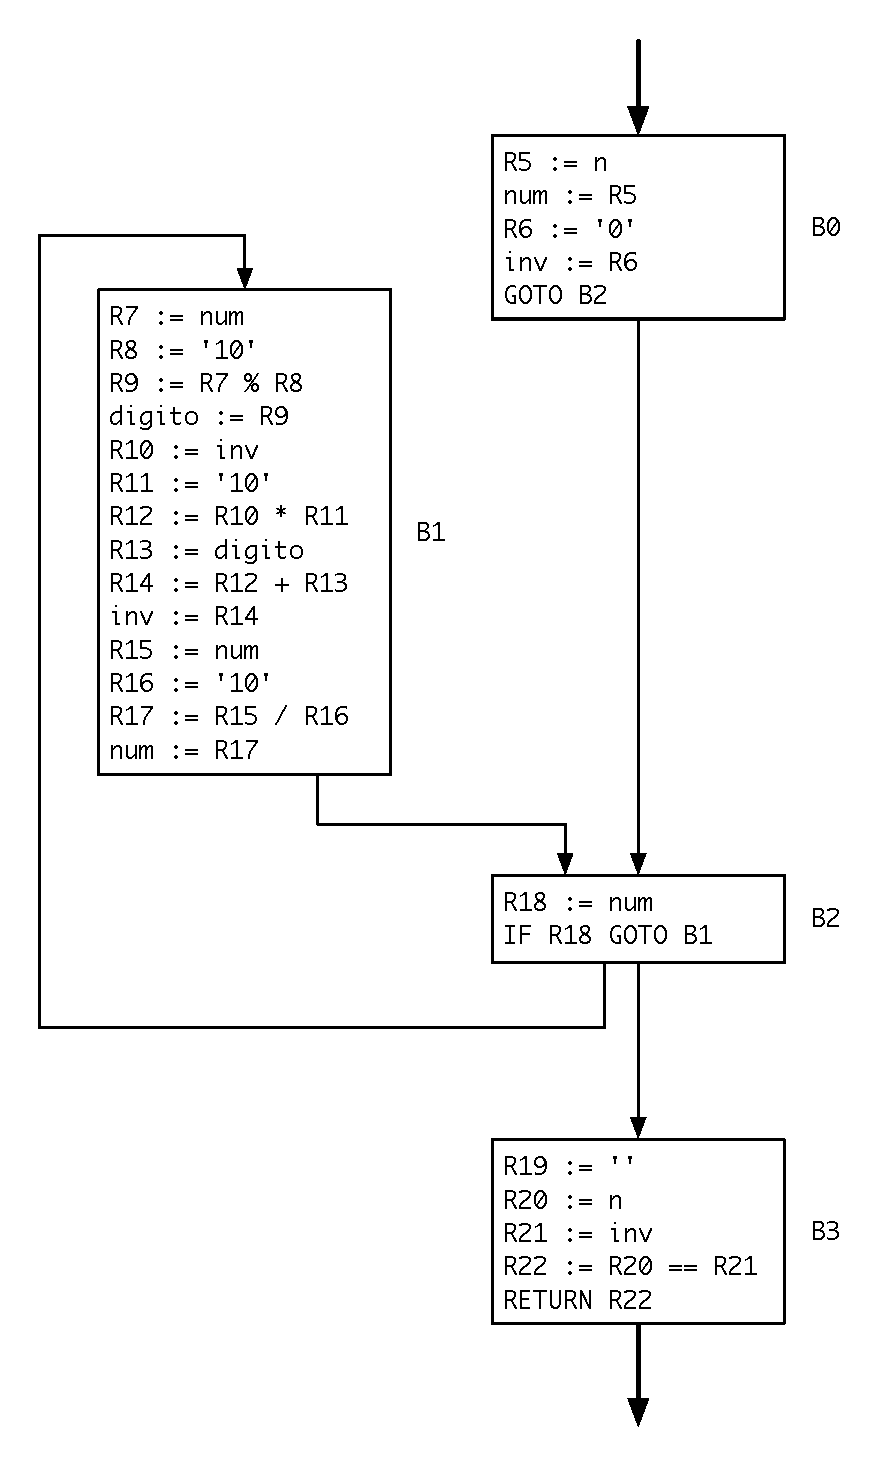
\includegraphics[scale=0.68]{figs/palindromo_bbs1}
  \caption{Blocos básicos e grafo de fluxo de controle construídos,
    etapa 1 \label{bbs}}
\end{figure}

Para se chegar a esta representação foi feita uma conversão de
máquina virtual baseada em pilha para algo semelhante a
uma máquina de infinitos registradores. Uma pilha temporária é
utilizada para simplificar essa transição, sendo acessada e atualizada
durante a construção de diversas instruções. Também são pré-alocados
registradores virtuais para as variáveis locais. A implementação da
\texttt{Tcl} disponibiliza uma lista dinâmica com todas as
variáveis locais, incluindo também os parâmetros formais da função,
sendo necessário apenas atribuir índices a elas. Os registradores que se
enquadram nessa lista tiveram seus nomes alterados para simplificar a
visualização. O registrador \verb!R1! foi renomeado para \verb!n! na
Figura \ref{bbs}, \verb!R2! para \verb!num!, \verb!R3! para \verb!inv!
e \verb!R4! para \verb!digito!.

Diversas instruções de atribuição recebem um
valor que se parece com número, como \verb!'0'! ou \verb!'10'!, mas
que estão sendo representados como \textit{strings}. Na realidade esses valores
são ponteiros para uma estrutura \verb!Tcl_Obj!, podendo assumir
qualquer tipo interno presente na linguagem. No exemplo anterior estes
dados realmente serão convertidos para inteiros. % A
%\textit{string} \verb!'puts'! armazenada no registrador 4 servirá como chave em uma tabela \textit{hash} que possui como valor a
%respectiva função (ou não, gerando um erro).
Todos esses ponteiros
estarão armazenados em um \textit{array} quando a função for executada,
sendo necessário definir os campos \verb!flags! e \verb!offset! da
estrutura \verb!Value! correspondente.
%O número entre parênteses na instrução \verb!CALL!
%indica que haverá 1 parâmetro na chamada e, no caso, este será o
%conteúdo de \verb!R9!.
%A única instrução no bloco de saída B3 indica o
%valor de retorno de função -- uma \textit{string} vazia.

Após construir os blocos básicos iniciais (Figura \ref{bbs}), uma
segunda etapa de construção é realizada. Nesta fase, as quádruplas que
tiverem operandos \verb!Tcl_Obj! serão
movidas para um bloco básico ``especial'' e, ainda, aquelas que
operarem sobre um parâmetro serão também copiadas para esse novo bloco
e a quádrupla original será ajustada. Essa etapa foi desenvolvida
baseando-se na observação de como os
\textit{bytecodes} são interpretados. Na Figura \ref{bbs}, todos
os \verb!Tcl_Obj! presentes são oriundos do \textit{array} de objetos
literais (Seção \ref{ambientexec1}). Carregar estes elementos têm um
custo tanto em quantidade de \textit{bytes} produzidos quanto no
desempenho do código nativo. No bloco básico 1, pode-se ver que há 3
movimentações de objetos literais (representado por '10'). Nos blocos 0 e 3
há dois acessos envolvendo o parâmetro formal. É mais simples
realizar movimentação entre registradores do que acessar o '10'
por meio de um \textit{array} que precisará ser percorrido a cada
iteração do laço. De modo semelhante, é mais eficiente primeiramente
carregar o valor recebido em um parâmetro para um registrador e operar
sobre ele do que buscar
seu valor atual no \textit{array} de variáveis locais. Com essas
transformações, a representação atualizada é exibida na Figura \ref{bbs2}.

\begin{figure}[ht!]
  \centering
  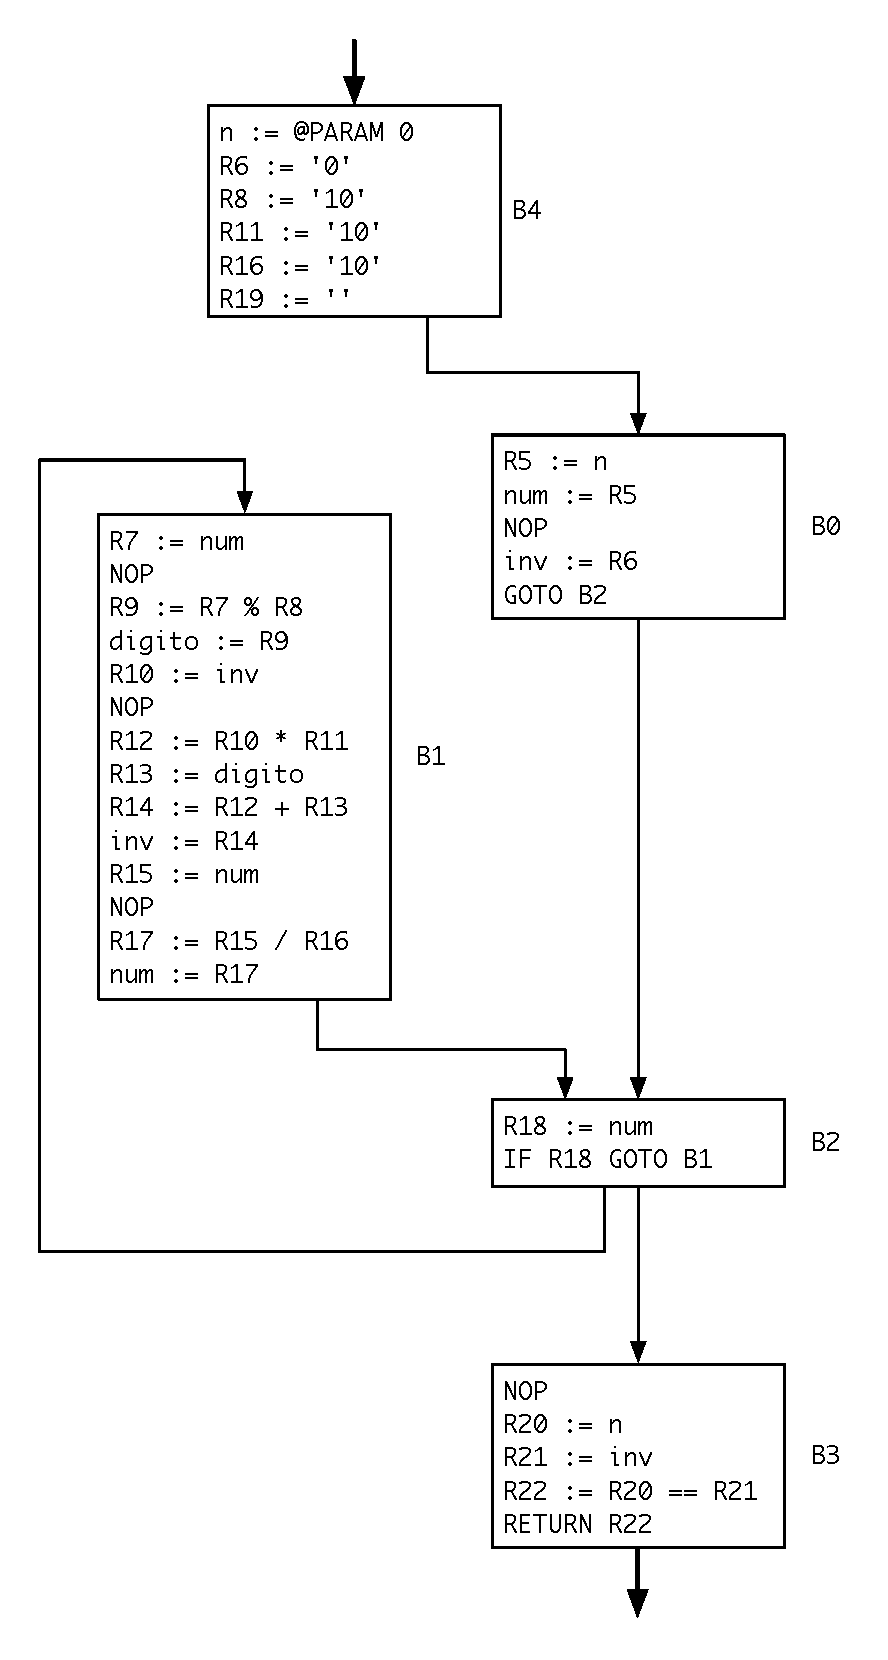
\includegraphics[scale=0.68]{figs/palindromo_bbs2}
  \caption{Blocos básicos e grafo de fluxo de controle final\label{bbs2}}
\end{figure}

Na Figura \ref{bbs2}, o bloco básico chamado de ``especial'' tornou-se
o bloco inicial. A primeira quádrupla ali contida indica que o
parâmetro na posição 0 do \textit{array} de variáveis locais deve ser
carregada para um registrador onde $n$ vive. As instruções \verb!NOP!
ficam a cargo do gerador de código decidir entre emitir código para
cada uma ou não. Essa segunda etapa traz ainda outro benefício. Se um
objeto \verb!Tcl_Obj! não puder ser transformado para um número
inteiro, então logo no primeiro bloco essa situação é detectada. Isso
permite que a volta ao interpretador ocorra de forma mais rápida.
% Com essa representação final surge outra oportunidade
%de otimização, ... olha só o R6, R8, R11 e R16 tudo com o mesmo
%objeto.. poderia utilizar só um.

O código da Figura \ref{fig:gray} utiliza 107 \textit{bytecodes}, aqui
(Figura \ref{bbs2}) representado com 32 quádruplas.
%Haviam 55 \textit{bytecodes} (não exibidos aqui) sendo utilizados para
%representar o código da figura \ref{fig:gray}, e agora 18 quádruplas
%são empregadas com o mesmo resultado. Nessa quantidade numérica
%superior destaca-se o uso de 9 bytes para representar a instrução
%\verb!INST_START_CMD! da \texttt{Tcl}, destinando 1 byte para o código
%da instrução em si, 4 bytes para indicar a posição relativa do início
%do próximo comando e
%4 bytes para contar a quantidade de comandos que fazem parte desse que
%está iniciando de modo a possibilitar ao  interpretador respeitar
%limites impostos para certos recursos por meio de
%APIs específicas. Porém,
Apesar das quádruplas estarem em número inferior,
%levando em conta o total de bytes contidos em cada quádrupla (de
%acordo com as estruturas acima) tem-se que
o consumo de memória é bastante superior (mas temporário), pois após
a geração de código as quádruplas não precisam mais estar em memória.
%Ao mesmo tempo é possível observar que muitas delas são passíveis a
Além disto, algumas são passíveis a
eliminação, ficando a cargo desta eliminação etapas de otimização.
 % otimizações em etapas futuras.

%Um último esclarecimento a respeito da figura \ref{bbs} precisa ser feito.
Os \textit{bytecodes} de desvio emitidos pela \texttt{Tcl} utilizam
operandos que descrevem posições relativas (negativas ou positivas) à
posição atual, porém, na
representação utilizada há somente desvios absolutos para blocos
básicos. Para essa tarefa cada
\textit{bytecode} é mapeado para cada bloco básico antes da construção do
conteúdo dos blocos, assumindo que não existirão mais quádruplas do que
\textit{bytecodes}.

\subsubsection{Mapeamento de alguns \textit{bytecodes} para quádruplas}

A seguir é realizada uma breve análise de como alguns
\textit{bytecodes} são convertidos para quádruplas. O exemplo da
Figura \ref{fig:limiar} é tomado como base para a discussão.

% XXX ?? Erro com tabular e language=Tcl
\begin{figure}[h]
  \centering
  \begin{tabular}{c}
    \begin{lstlisting}%[language=Tcl]

proc limiar-bipolar {x} {
  if {$x >= 0} {
    return 1
  } else {
    return -1
  }
}
    \end{lstlisting}
  \end{tabular}
  \caption{Procedimento exemplo para análise \textit{bytecodes}
    $\rightarrow$ quádruplas\label{fig:limiar}}
\label{xx$xx}
\end{figure}

%Ao executar tal código o interpretador gera uma exceção. Porém, antes de
%exibir a descrição do problema, a função \verb!JIT_Compile! é
%invocada (assumindo que \verb!JIT_REQINVOKE! ainda está definida em \verb!0!).
A Tabela \ref{tabela1} apresenta, lado a lado, os \textit{bytecodes}
produzidos pela \texttt{Tcl} e o código intermediário gerado pelo
compilador JIT para o procedimento
da Figura \ref{fig:limiar}. Para simplificar a visualização dos
\textit{bytecodes}, fez-se uso de \textit{labels} que não existem no
código produzido pela \texttt{Tcl}.

\begin{table}[h]
  \centering
  \caption{Saída produzida para procedimento da Figura \ref{fig:limiar} \label{tabela1}}
  \begin{tabular}{| p{4cm} | p{4cm} |}
    \hline
    \bf{Bytecode} & \bf{Registradores} \\
\begin{verbatim}
LOAD_SCALAR x
PUSH '0'
GE
JUMP_FALSE label1

START_CMD
PUSH '1'
DONE
JUMP label2

label1: START_CMD
PUSH '-1'
DONE

label2: DONE
\end{verbatim} &
\begin{verbatim}
R2 := x
R3 := '0'
R4 := R2 >= R3
IF NOT R4 GOTO B2


R5 := '1'
RETURN R5
GOTO B3

B2:
R6 := '-1'
RETURN R6

B3:
\end{verbatim} \\
    \hline
  \end{tabular}
\end{table}

%Os registradores R2 e R3 contém endereços de memória
%estruturados como \verb!Tcl_Obj!. Por esse motivo, não
%há um endereço previsto para a variável \verb!x! e, portanto, esse
%código certamente geraria um erro se fosse compilado para código de
%máquina.%  Corrigindo,
% alterando para imprimir \verb!$::x!, a seguinte sequência de bytecodes
% e de registradores é produzida:

% \begin{table}[h]
%   \centering
%   \caption{Saída produzida para procedimento corrigido da figura 5}
%   \begin{tabular}{| p{4cm} | p{4cm} |}
%     \hline
%     \bf{Bytecode} & \bf{Registradores} \\
% \begin{verbatim}
% PUSH 'puts'
% PUTS '::x'
% LOAD_SCALAR_STK
% INVOKESTK 2
% DONE
% \end{verbatim} &
% \begin{verbatim}
% R1 := 'puts'
% R2 := '::x'
% ...
% CALL R1 (1) R2
% \end{verbatim} \\
%     \hline
%   \end{tabular}
% \end{table}

%%% NEXT_INST_V(1, 1, 1)

%O processo de mapear um determinado \textit{bytecode} para quádruplas
%é simples. Este processo será descrito detalhando as informações
%contidas na Tabela \ref{tabela1}.

%Continuando ainda no exemplo da figura \ref{fig:global1}, detalhamos
%como o mapeamento de uma coluna para outra foi realizado no restante
%dessa seção. Começando pela
%A instrução \verb!DONE! %vemos que nada equivalente aparece na coluna
%a direita.  por exceções e tão pouco
%por código de retorno anormal -- embora tais tarefas sejam realizadas em
%diversos pontos da máquina virtual..

O lado direito da Tabela \ref{tabela1} representa o resultado da etapa
1 da construção de CFG, o resultado final da etapa 2 não auxiliaria no
propósito desaa discussão.

A instrução \verb!START_CMD!
não possui uma quádrupla equivalente. Isso é resultado da
atual simplificação feita. Diferentemente
da máquina virtual, o código nativo não verifica se o procedimento
sendo executado foi alterado e simplesmente assume que isso não
ocorrerá.

A instrução \verb!PUSH! é mapeada utilizando uma pilha temporária e
um \textit{array} de objetos literais. Um operando que segue a
instrução \verb!PUSH! é tomado como o índice do \textit{array}.
O registrador criado neste ponto,
\verb!R3! no exemplo, é então empilhado. A instrução \verb!LOAD_SCALAR!
é mapeada de forma similar, mas ela se baseia em obter o
endereço da variável escalar de uma lista de variáveis locais
criada pelo compilador da \texttt{Tcl} para o procedimento
corrente. Neste ponto os registradores R2 e R3 estão na pilha e
a instrução \verb!GE! deve ser convertida. Típico de uma máquina de
pilha, esta instrução não requer que ela seja seguido de operandos
pois os mesmos equivalem aos dois últimos empilhados. Da mesma forma,
a pilha artificial criada é utilizada para simular esse comportamento.
O resultado da comparação é empilhado, mas a representação utilizada
pelo compilador dinâmico também requer que tal resultado seja
armazenado em um novo registrador.

Para converter a instrução de desvio \verb!JUMP_FALSE!, a pilha
utilizada é consultada para descobrir qual registrador contém um valor
que determina a realização do desvio ou não. O destino é calculado
utilizando o mapeamento mencionado no final da Seção \ref{intermediate}.

% Seguida de um
%operando, chamado de \verb!objc!, indicando a quantidade total de
%argumentos (incluindo o nome da função) os elementos
%$0 \dots objc - 2$ da pilha a partir do topo são os parâmetros para
%a função na posição $objc - 1$ a partir do topo. Na representação
%utilizada não é considerado o nome da função como um parâmetro, por isso
%entre parênteses está o número 1 ao invés do 2.
A instrução \verb!DONE! é utilizada para indicar um ponto de
retorno, sua conversão para o modelo de registradores consiste
simplesmente em retornar o último objeto empilhado. Nota-se que a
última instrução
não teve código produzido, isso é devido a uma heurística aplicada de
que uma sequencia de instruções \verb!DONE! equivale a uma única.

\subsection{Geração de Código de Máquina}
\label{codegen}
Após descrever como a representação intermediária é construída e
o funcionamento do sistema para
executar o código gerado, o próximo passo é descrever como tal
código de máquina é gerado considerando o uso de uma arquitetura CISC
(\textit{Complex Instruction Set Computer}) e, em específico, a
IA-32 \cite{intel_basicarch}.
\nomenclature{CISC}{Complex Instruction Set Computer}

%Logo após a criação do CFG, a função \verb!JIT_CodeGen! é invocada e o
%seu resultado é um ponteiro para \verb!unsigned char! que em seguida é
%passado para um campo \verb!ncode! de um procedimento específico. A
%função \verb!JIT_CodeGen! faz todo o trabalho que cabe a
%esta seção.

\subsubsection{Reservando e controlando espaço para os bytes}
%A primeira questão a ser tratada é onde colocar os bytes que serão
Um ponto importante é decidir onde armazenar os bytes que serão
gerados. De acordo com a Seção \ref{codeexec}, uma função é apenas uma
sequência de bytes que pode ser executada. De forma direta é possível
pensar em armazenar os bytes em um região de memória alocada por
uma função como \verb!malloc!. Porém, simplesmente fazer isso não garante
que o sistema operacional permitirá a execução desta sequência de bytes.

Com a introdução do bit NX (\textit{No-eXecute}) pela AMD e depois
pela Intel (que renomeou para \textit{eXecute-Disable}), o hardware
passou a prevenir a execução de código em páginas destinadas a
dados \cite{intel_prog} e, dessa forma, eliminar
parcialmente ataques relacionados a \textit{buffer
  overflow}\footnote{O artigo ``Code Injection Attacks on
  Harvard-Architecture Devices'' de Aurélien Francillon e Claude
  Castelluccia publicado na ACM CCS 2008 menciona trabalhos que
  contornam a proteção por bit NX além de outras proteções que
  tem sido desenvolvidas.}.
Por essa razão uma região de
memória alocada por meio do \verb!malloc! não poderá ter seu conteúdo
executado em sistemas que fazem uso desse recurso. Uma forma de
contornar esse problema é utilizar a função \verb!mprotect!,
definindo a região com proteção de leitura e execução após escrever os dados
desejados. Entretanto, essa função requer que o tamanho da região
alocada seja um múltiplo do tamanho de página -- denominado de
\textit{page-aligned}. Para contornar este outro problema é possível
utilizar a função
\verb!memalign! ou \verb!valloc!, de acordo com a disponibilidade. Porém,
o mais adequado é definir o tamanho da região como um múltiplo do
tamanho de página, eliminando a necessidade de alinhamento e reduzindo
questões de portabilidade. % A quantidade de bytes que define o tamanho
%de uma página pode ser obtido com a função
%\verb!getpagesize!.
A estrutura exibida na Figura \ref{mcode-struct}
juntamente com as funções% \verb!pagesize!, \verb!newpage! e
%\verb!pagenowrite!
 exibidas no Apêndice \ref{apendiceA}
tratam dos problemas mencionados %de forma similar a descrita
 e também
de questões de portabilidade entre os sistemais operacionais Windows e UNIX.

\begin{figure}[h]
  \centering
  \begin{tabular}{c}
    \begin{lstlisting}[language=C]
struct MCode {
  unsigned char *mcode, *codeEnd;
  int limit, used;
};
    \end{lstlisting}
  \end{tabular}
  \caption{Estrutura para controlar uso de memória do código gerado\label{mcode-struct}}
\end{figure}

Os campos \verb!limit! e \verb!used! determinam o tamanho total
alocado e o espaço usado até o momento, respectivamente. Atingindo o
valor limite, uma nova página precisa ser alocada e o campo
\verb!limit! tem seu valor dobrado. Os campos \verb!mcode! e
\verb!codeEnd! apontam para o início do código de máquina e o
ponto atual na região de memória, respectivamente. O endereço contido em
\verb!mcode! é o que será instalado no campo
\verb!ncode! da estrutura \verb!JIT_Proc! de um procedimento
específico caso a geração de código tenha sucesso.


\subsubsection{Início e término da geração}
\label{begin-end-codegen}

Antes de gerar código específico para um CFG, é gerado um prólogo
genérico que pode ser visto na 
Figura \ref{prologo-epilogo}. Após a geração de código para o CFG é
gerado um epílogo que também é
apresentado na Figura \ref{prologo-epilogo}. O código gerado pode
lidar com registros de ativação de tamanho variado, por isso é
definido um ponto base para acessar
% A divisão da pilha em
%partes (\textit{frames}) origina o conceito de \textit{stack frame}
%que é manuseado pelo código do prólogo. Cada \textit{stack frame} pode
%variar de tamanho, e por isso definimos um ponto base para acessar
parâmetros ou variáveis locais de forma que seja respeitada as
condições da ABI \cite{systemv-abi}. Essa base, ou ponto de
referência, fica definida como 
o endereço contido no registrador \verb!ebp! após a execução do
prólogo. É possível encontrar definições de prólogo que incluam código
para salvar os registradores \verb!ebx!, \verb!edi!, \verb!esi!
e \verb!esp! uma vez que, de acordo com a ABI seguida, esses
registradores (além do \verb!ebp! que já é salvo) precisam ser
preservados entre chamadas. Na
implementação atual, código para salvar qualquer um desses
registradores precisa ser gerado conforme necessário. O epílogo possui
código antônimo daquele contido no prólogo, efetivamente desfazendo o
registro de ativação construído e retornando para o endereço contido
na topo da pilha corrente.

\begin{figure}[ht!]
  \centering
  \begin{lstlisting}[language=C, numbers=left]
#define PROLOGUE(code, stsize) {  \
  PUSH_REG(code, EBP); \
  MOV_REG_REG(code, ESP, EBP) \
  if (stsize > 0) { \
    if (4 * stsize > 127) { SUB_IMM32_REG(code, 4 * stsize, ESP); } \
    else { SUB_IMM8_REG(code, 4 * stsize, ESP); } \
  } \
}

#define EPILOGUE(code, stsize) { \
  if (stsize > 0) { \
    if (4 * stsize > 127) { ADD_IMM32_REG(code, 4 * stsize, ESP); } \
    else { ADD_IMM8_REG(code, 4 * stsize, ESP); } \
  } \
  LEAVE(code); RETN(code) \
}

#define PUSH_REG(code, reg) *code++ = 0x50 + reg
#define MOV_REG_REG(code, src, dest) \
    *code++ = 0x89;                  \
    *code++ = MODRM(0x3, src, dest)
#define LEAVE(code) *code++ = 0xC9
#define RETN(code) *code++ = 0xC3

#define ADD_IMM8_REG(code, imm, reg) \
    *code++ = 0x83; \
    *code++ = MODRM(0x3, 0, reg); \
    *code++ = imm
#define ADD_IMM32_REG(code, imm, reg) \
    *code++ = 0x81; \
    *code++ = MODRM(0x3, 0, reg); \
    IMM32(code, imm)
#define SUB_IMM8_REG(code, imm, reg) \
    *code++ = 0x83; \
    *code++ = MODRM(0x3, 0x5, reg); \
    *code++ = imm
#define SUB_IMM32_REG(code, imm, reg) \
    *code++ = 0x81; \
    *code++ = MODRM(0x3, 0x5, reg); \
    IMM32(code, imm)

#define MODRM(mod, reg, rm) (mod << 6) + (reg << 3) + rm

#define IMM32(code, v) \
    *code++ = v; *code++ = v >> 8; \
    *code++ = v >> 16; *code++ = v >> 24
  \end{lstlisting}
  \caption{Código completo para epílogo e prólogo em x86\label{prologo-epilogo}}
\end{figure}

Para os códigos exibidos adiante assume-se que \verb!code! seja um
ponteiro da forma do \verb!codeEnd!
da estrutura \verb!MCode! (Figura \ref{mcode-struct}) e disponha de
uma região de memória suficiente para a execução correta dessas macros.

Na Figura \ref{prologo-epilogo}, o código entre as linhas 1 e 16, é
semelhante com código em \texttt{Assembly} \cite{assembly1} de sintaxe
AT\&T \cite{sintaxeatt}. A partir da linha 18 é semelhante, porém
simplificado, a um montador para x86. Para entender o significado das
linhas 18, 20, 21 e 42, a Tabela \ref{mov-push-1} apresenta uma descrição
sucinta das instruções \verb!MOV! e \verb!PUSH!.
% com formato
%similar àquelas encontradas nos  manuais da Intel
%\cite{intel_aam}\cite{intel_naz} mas
%adaptada para sintaxe AT\&T e reduzida para as necessidades da situação.

\begin{table}[ht!]
  \caption{Uma variação das instruções MOV e PUSH\label{mov-push-1}}
  \centering
  \begin{tabular}{l l l l c}
    \toprule
    Opcode  & Instrução     & Operando 1    & Operando 2    &  Modo 64-Bits \\
    \midrule
    0x89 /r & \verb!MOV r32, r/m32!& ModRM:reg (r) & ModRM:r/m (w) &  Válido       \\
    0x50+rd & \verb!PUSH r32!      & reg (r)       &               &  N.C.         \\
    \bottomrule
  \end{tabular}
\end{table}

A coluna ``\textit{Opcode}'' apresenta
os códigos hexadecimais das variações de \verb!MOV! e \verb!PUSH!
utilizadas e também as informações ``/r'' e ``+rd''. A primeira
indica que a instrução faz uso de um byte chamado de ModR/M, que é
dividido em três partes: mod (2 bits),
reg/opcode (3 bits) e r/m (3 bits), da direita para esquerda seguindo
a ordem \textit{little-endian}. O formato final do byte é formado conforme
a linha 13 da Figura \ref{prologo-epilogo}.
A parte ``reg/opcode'' determina ou um
número de registrador ou mais três bits de informação de acordo com
a especificação do \textit{opcode} (que não é utilizado aqui). O campo
``r/m'' ou específica um registrador como um operando ou pode ser
combinado com o ``mod'' para codificar um modo de endereçamento. Para
mais detalhes sobre o byte ModR/M recomenda-se a consulta ao manual da
\citeonline[capítulo 2]{intel_aam}. Além disto,
a informação ``+rd'' indica que um código entre 0
e 7, simbolizando um registrador de 32 bits, deve ser somado ao valor
em hexadecimal. A segunda coluna indica que os operandos são
registradores de 32 bits (\verb!r32!) ou que pode-se buscar algum
conteúdo no endereço de memória calculado (\verb!r/m32!). No
caso dessa variação do \verb!MOV! o objetivo é mover dados de um
registrador para outro. A última coluna da tabela indica se o
\textit{opcode} apresentado pode ser utilizado no modo 64-bits ou não;
no caso do \verb!PUSH! está indicado que a sintaxe da instrução
não é codificável no modo 64-bits. Ou seja, essa última coluna
indica quais das instruções atualmente codificadas pelo
compilador teriam que ser no mínimo ajustadas para gerar código para
uma arquitetura x64.

A informação contida entre parênteses ``r'' ou ``w'', indica
que o conteúdo do operando será lido
(\textit{\textbf{r}ead}) ou atualizado
(\textit{\textbf{w}ritten}) pelo processador.
 Para a instrução \verb!MOV! é possível utilizar 32 combinações de
endereçamento, devido ao uso do byte ModR/M. Entretanto, o interesse é
apenas na especificação de registradores. De acordo com a
Tabela 2.2 do manual em \citeonline[seção 2.1.5]{intel_aam}
é necessário estabelecer o campo ``mod'' do byte ModR/M em 3 para
essa situação e, assim, juntamente com os números dos registradores fonte e
destino é possível completar esse byte adicional. Dessa forma, a
linha 9 do código da Figura \ref{prologo-epilogo} está resolvida.


\subsubsection{Percorrendo Blocos e Gerando Código}

O gerador de código percorre os blocos básicos do CFG por meio de uma
busca em profundidade e emite código para as instruções contidas em
cada bloco. Durante o percurso do CFG, cada quádrupla
do bloco básico corrente é acessada e um
\textit{switch} de instruções define qual cláusula corresponde a
instrução contida na quádrupla.

Devido a granularidade alta, imposta pela representação intermediária
atual, mesmo instruções simples requerem uma quantidade
relativamente alta de \textit{bytes} para codificá-las. Para realizar
uma discussão detalhada, faz-se uso de uma única instrução de
multiplicação.

O exemplo da Figura \ref{myinc} gera 2 blocos básicos com um total de 5
quádruplas, o processo de tradução de \textit{bytecodes} é exibido na
Tabela \ref{tabela-processo}.

% XXX ?? Erro estranho se deixar language=Tcl
\begin{figure}[ht!]
  \centering
  \begin{tabular}{c}
    \begin{lstlisting}%[language=Tcl]

proc twice {x} {
  expr {$x * $x}
}
    \end{lstlisting}
  \end{tabular}
  \caption{Código exemplo para análise da geração de código \label{myinc}}
\end{figure}

\begin{table}[ht!]
  \centering
  \caption{Processo de conversão do código da Figura \ref{myinc} \label{tabela-processo}}
  \begin{tabular}{| p{2.8cm} | p{3.3cm} | p{3.4cm} | p{5cm} |}
    \hline
    \bf{Bytecode} & \bf{CFG, etapa 1} & \bf{CFG, etapa 2} & \bf{Instruções}\\
\begin{verbatim}
LOAD_SCALAR x
LOAD_SCALAR x
MULT
DONE
\end{verbatim} &
\begin{verbatim}
BB0:
  R2 := x
  R3 := x
  R4 := R2 * R3
  RETURN R4
\end{verbatim} &
\begin{verbatim}
BB1:
  R1 := @PARAM 0
BB0:
  R2 := R1
  R3 := R1
  R4 := R2 * R3
  RETURN R4
\end{verbatim} &
\begin{verbatim}
LOAD_SCALAR src, dest
JIT_INST_MOVE src, dest
JIT_INST_MOVE src, dest
INST_MULT s1, s2, dest
JIT_INST_SAVE src
\end{verbatim} \\
    \hline
  \end{tabular}
\end{table}

A última coluna da Tabela \ref{tabela-processo} identifica as
instruções representantes de cada quádrupla.
Os nomes das instruções que não
começam com \verb!JIT_! foram reaproveitados da \texttt{Tcl}.
Outra informação contida
diz respeito a quantidade de \textit{bytes} a serem reservados na
pilha, definindo o parâmetro \verb!stsize! para o código do prólogo e
epílogo da Figura \ref{prologo-epilogo}. Por tratar-se de um compilador não
otimizador, também não é aplicado uma fase de alocação de
registradores. Por isso, cada registrador virtual é mapeado para um
endereço na pilha e seus endereços são derivados a partir do seu
número exibido nas figuras anteriores.

Ao encontrar uma instrução \verb!LOAD_SCALAR!, o gerador de código
sabe que precisará armazenar uma variável local em uma posição da
pilha. A Seção \ref{codeexec} descreveu a assinatura
da função criada pelo compilador JIT, sem detalhar os tipos dos argumentos.
Para manter a compatibilidade com as estruturas internas do ambiente de
execução, o primeiro parâmetro é uma estrutura
interna \verb!Interp! que será utilizada para acessar a
variável local. A partir desta informação, os \textit{bytes} gerados que
imediatamente seguem o prológo gerado são referentes a movimentação do
primeiro parâmetro para um registrador. O código na Figura
\ref{copy-param} realiza essa primeira função de acordo com a ABI escolhida.


\begin{figure}[ht!]
  \centering
  \begin{tabular}{c}
    \begin{lstlisting}[language=C]
#define COPY_PARAM_REG(code, paramn, reg) \
  MOV_DISP8DREG_REG(code, 8 + 4 * paramn, EBP, reg)

#define MOV_DISP8DREG_REG(code, disp, src, dest) \
  *code++ = 0x8B;                              \
  *code++ = MODRM(0x1, dest, src);             \
  *code++ = disp
    \end{lstlisting}
  \end{tabular}
  \caption{Cópia de parâmetro para registrador seguindo ABI escolhida\label{copy-param}}
\end{figure}

Assumindo um uso da forma:
\verb!COPY_PARAM_REG(code, 0, EAX)!, será possível encontrar em tempo de 
execução o endereço de uma estrutura \verb!Interp! no registrador 
\verb!eax!. Vale ressaltar o uso de outra variação
da instrução
\verb!MOV! aqui (em complemento àquela da Tabela \ref{mov-push-1}),
 que é traduzida para \texttt{Assembly} como:
\verb!movl disp(%src), %dest!. Nesse ponto é possível atravessar a
estrutura \verb!Interp! até
alcançar o \textit{array} que contém todas as variáveis locais, utilizando
trecho de código apresentado na Figura \ref{goto-varstruct}.

\begin{figure}[ht!]
  \centering
  \begin{tabular}{c}
    \begin{lstlisting}[language=C]
long int offset;
offset = offsetof(Interp, varFramePtr);
MOV_DISP8DREG_REG(code, offset, EAX, EAX);
offset = offsetof(CallFrame, compiledLocals);
MOV_DISP8DREG_REG(code, offset, EAX, EAX);
    \end{lstlisting}
  \end{tabular}
  \caption{Percorrendo Interp até variáveis locais\label{goto-varstruct}}
\end{figure}


A estrutura \verb!Interp! possui o campo \verb!varFramePtr! que
aponta para um \verb!CallFrame!. 
A estrutura \verb!CallFrame!, por sua vez, possui um
\verb!array! de tipo \verb!Var!, chamado de \verb!compiledLocals!,
que armazena as variáveis locais. Portanto, a Figura
\ref{goto-varstruct} gera código equivalente a:
\verb!interp->varFramePtr->compiledLocals!, assumindo
que \verb!interp! aponte para o parâmetro de tipo
\verb!Interp!. Após isso, é utilizado o campo
\verb!offset! da estrutura \verb!Value! de \verb!src_a!, deslocando em
\verb!compiledLocals! até o ponto desejado e tornando possível acessar
o \verb!Tcl_Obj! que representa a variável local procurada (código
apresentado na Figura \ref{goto-localvar}, que é a continuação do
código da Figura \ref{goto-varstruct}). A
variável é um parâmetro para a função
escrita em \texttt{Tcl}. Além disso, é o primeiro argumento e, por
essa razão, o deslocamento será 0 no \verb!array! \verb!compiledLocals!.

\begin{figure}[h]
  \centering
  \begin{tabular}{c}
    \begin{lstlisting}[language=C]
#define ADD_IMM8_REG(code, imm, reg) \
  *code++ = 0x83;                  \
  *code++ = MODRM(0x3, 0, reg);    \
  *code++ = imm


if (src_a->offset) {
  ADD_IMM8_REG(code, sizeof(Var) * src_a->offset, EAX);
}
offset = offsetof(Var, value.objPtr);
MOV_DISP8DREG_REG(code, offset, EAX, EAX);
    \end{lstlisting}
  \end{tabular}
  \caption{Acessando variável local\label{goto-localvar}}
\end{figure}

Após acessar o objeto desejado, é possível obter o valor inteiro
contido no mesmo (se houver). Objetos \verb!Tcl_Obj! contém uma
estrutura responsável por armazenar o valor inteiro (assim como os
demais tipos existentes), mas não há
garantias de que o mesmo contenha um valor válido mesmo se o objeto
``parecer'' ser um número. Por essa razão, é necessário fazer uso da
função \verb!Tcl_GetLongFromObj! que verifica se a representação em
\textit{bytes} do objeto pode ser convertida para um inteiro e, então,
atualiza a sua representação interna mais eficiente com o valor
obtido. Sendo assim, e seguindo o modelo simplificado mencionado no
ínicio da Seção \ref{sistemacompilacao}, a conclusão da codificação da
instrução \verb!LOAD_SCALAR! requer uma chamada a
\verb!Tcl_GetLongFromObj!, verificação de erro e armazenamento do
valor obtido. A Figura \ref{fimloadscalar} apresenta o código
utilizado neste momento.

%  Entretanto, o endereço desse objeto será
% reutilizado antes do código de máquina terminar e, portanto, é
% necessário salvá-lo
% em outro registrador (se possível). O código na
% Figura \ref{inc-tclobj} avança até o ponto em que o valor contido no
% objeto é incrementado, simplificações são feitas de modo que é
% assumido que o objeto já construiu uma representação de tipo inteiro.

\begin{figure}[h]
  \centering
  \begin{tabular}{c}
    \begin{lstlisting}[language=C]
AND_IMM8_REG(code, -16, ESP); /* Alinhamento */
PUSH_REG(code, EBX);          /* calle-save  */

/* End. mem. para armazenar valor inteiro. */
LEA_DISP8DREG_REG(code, staddr, EBP, EDX);

PUSH_REG(code, EDX);          /* End. armaz. valor */
PUSH_REG(code, EAX);          /* (Tcl_Obj *) */
PUSH_DISP8DREG(code, 8, EBP); /* (Interp *) */

MOV_IMM32_REG(code, (ptrdiff_t)Tcl_GetLongFromObj, EBX);
CALL_ABSOLUTE_REG(code, EBX);

ADD_IMM8_REG(code, 12, ESP);
POP_REG(code, EBX);

/* Verificar por cod. retorno. */
CMP_IMM8_REG(code, 0, EAX);
JUMP_NOTEQ(code, ``LINTERP'');
    \end{lstlisting}
  \end{tabular}
  \caption{Conclusão da instrução LOAD\_SCALAR \label{fimloadscalar}}
\end{figure}

Na Figura \ref{fimloadscalar}, o variável \verb!staddr!
refere-se a um endereço na pilha calculado por meio campo
\verb!offset! do registrador virtual. O alinhamento da pilha à 16
\textit{bytes} é feito por causa da ABI do sistema operacional Mac OS
X \cite{macosx-abi}, que exige este alinhamento para chamadas de
funções mesmo na arquitetura IA-32. Um outro ponto a considerar neste
código, é a verificação de código de erro. Esse rótulo \verb!LINTERP!
(última linha da Figura \ref{fimloadscalar})
aparece logo abaixo do epílogo criado inicialmente (Subseção
\ref{begin-end-codegen}), agindo como um
outro epílogo mas que define o conteúdo do registrador \verb!eax! como
sendo \verb!JIT_RESULT_INTERPRET!. Quando essa posição do código é
atingida, significa que a suposição de que os valores seriam inteiros
falhou e o código deve ser interpretado pela TVM.

As duas instruções \verb!JIT_INST_MOVE! que seguem são mais simples de
serem codificadas. Cada uma realiza apenas a movimentação do conteúdo de
um endereço de pilha para outro endereço de pilha, fazendo uso de duas
instruções \verb!MOV!.

A instrução \verb!INST_MULT! carrega o conteúdo de dois endereços de
pilha para registradores, aplica a instrução \verb!IMUL! e
armazena o resultado na posição de pilha descrita pelo registrador
virtual de destino.

Nesse momento o resultado de $x^2$ foi calculado, mas existe a
necessidade de retornar esse valor num formato aceito pelo restante do
ambiente. Essa é a tarefa da instrução \verb!JIT_INST_SAVE!.
De acordo com o funcionamento da \texttt{Tcl}, é
necessário definir o objeto resultado da função \verb!twice! para o
interpretador em que a função executa. Efetivamente não é feito
uso de interpretador aqui, entretanto é necessário armazenar
um objeto \verb!Tcl_Obj! em \verb!interp->objResultPtr! pois possívelmente será acessado
por outros comandos \texttt{Tcl} por meio da função \verb!Tcl_GetObjResult!.
Para preencher esse requerimento é feito uso da função
\verb!Tcl_NewLongObj! e \verb!Tcl_SetObjResult!. A primeira é
utilizada para criar um \verb!Tcl_Obj! com o valor resultante de
$x^2$, a segunda é responsável por armazenar o objeto criado pela
primeira no lugar adequado.
Somente depois dessas tarefas é possível
retornar o código \verb!TCL_OK! (\verb!0!) para indicar sucesso.
O código contido nas Figuras \ref{myinc-last-macros} e \ref{myinc-last}
realiza essas tarefas finais.

% Nesse momento a variável local já foi incrementada mas ainda
% existe a necessidade de realizar algumas tarefas antes de retornar. De
% acordo com o
% funcionamento da \texttt{Tcl}, é
% necessário definir o objeto resultado da função \verb!myinc! para o
% interpretador em que a função executa. Efetivamente não é feito
% uso de interpretador aqui, entretanto é necessário armazenar uma cópia desse
% \verb!Tcl_Obj! em \verb!interp->objResultPtr! pois possívelmente será acessado
% por outros comandos \texttt{Tcl} por meio da função \verb!Tcl_GetObjResult!.
% Para preencher esse requerimento é feito uso da função \verb!Tcl_SetObjResult!.
% Também é necessário atualizar a representação em
% \verb!string! do objeto incrementado, caso contrário um comando
% \verb!puts! exibiria o equivalente ao conteúdo existente antes do incremento.
% Depois dessas tarefas é possível
% retornar o código \verb!TCL_OK! (\verb!0!) para indicar sucesso.
% O código contido nas Figuras \ref{myinc-last-macros} e \ref{myinc-last}
% realiza essas tarefas finais.

\begin{figure}[ht!]
  \centering
  \begin{tabular}{c}
    \begin{lstlisting}[language=C]
#define PUSH_DISP8REG(code, disp, reg) \
  *code++ = 0xFF;                    \
  *code++ = MODRM(0x1, 6, reg);      \
  *code++ = disp
#define MOV_IMM32_REG(code, imm32, reg) \
  *code++ = 0xB8 + dest;              \
  IMM32(code, imm32)
#define CALL_ABSOLUTE_REG(code, reg) \
  *code++ = 0xFF;                  \
  *code++ = MODRM(0x3, 2, reg)
#define POP_REG(code, reg) *code++ = 0x58 + reg
#define XOR_REG_REG(code, src, dest) \
  *code++ = 0x33;                  \
  *code++ = MODRM(0x3, src, dest)

#define IMM32(code, v) \
  *code++ = v; *code++ = v >> 8; \
  *code++ = v >> 16; *code++ = v >> 24
    \end{lstlisting}
  \end{tabular}
  \caption{Macros adicionais requeridos pela Figura \ref{myinc-last}\label{myinc-last-macros}}
\end{figure}

\begin{figure}[ht!]
  \centering
  \begin{tabular}{c}
    \begin{lstlisting}[language=C]
MOV_DISP8DREG_REG(code,
    INDEX_TO_STACKADDR(VREG_OFFSET(src)), EBP, EDX);

/* Chamar Tcl_SetObjResult. */
PUSH_REG(code, EDX); /* Resultado de x * x. */
MOV_IMM32_REG(code, (ptrdiff_t)Tcl_NewLongObj, EAX);
CALL_ABSOLUTE_REG(code, EAX);
/* EAX recebeu o Tcl_Obj* resultante. */

PUSH_REG(code, EAX);
PUSH_DISP8DREG(code, 8, EXP); /* (Interp *) */
MOV_IMM32_REG(code, (ptrdiff_T)Tcl_SetObjResult, ECX);
CALL_ABSOLUTE_REG(code, ECX);

/* ``Remove'' 8(%ebp) e EAX da pilha. */
ADD_IMM8_REG(code, 4, ESP);

/* Retornar TCL_OK (ver ABI). */
XOR_REG_REG(code, EAX, EAX);
GOTO(code, ``LEAVE'');
    \end{lstlisting}
  \end{tabular}
  \caption{Tarefas finais para o código da Figura \ref{myinc}\label{myinc-last}}
\end{figure}

Após concluir a geração de código, a função
\verb!JIT_CodeGen! está pronta para encerrar; ajustando a permissão
das páginas utilizadas e retornando
o endereço inicial para a sequência de bytes gerada. %que pode ser executada
%como uma função.
Para o código da Figura \ref{myinc} foram gerados 120 \textit{bytes}.
O código de máquina para esse trecho é exibido na Tabela
\ref{codcompleto} na forma hexadecimal, \texttt{Assembly} e instruções
de nível médio, respectivamente.

\begin{table}[ht!]
  \centering
  \caption{Visualização do código gerado para Figura \ref{myinc} \label{codcompleto}}
  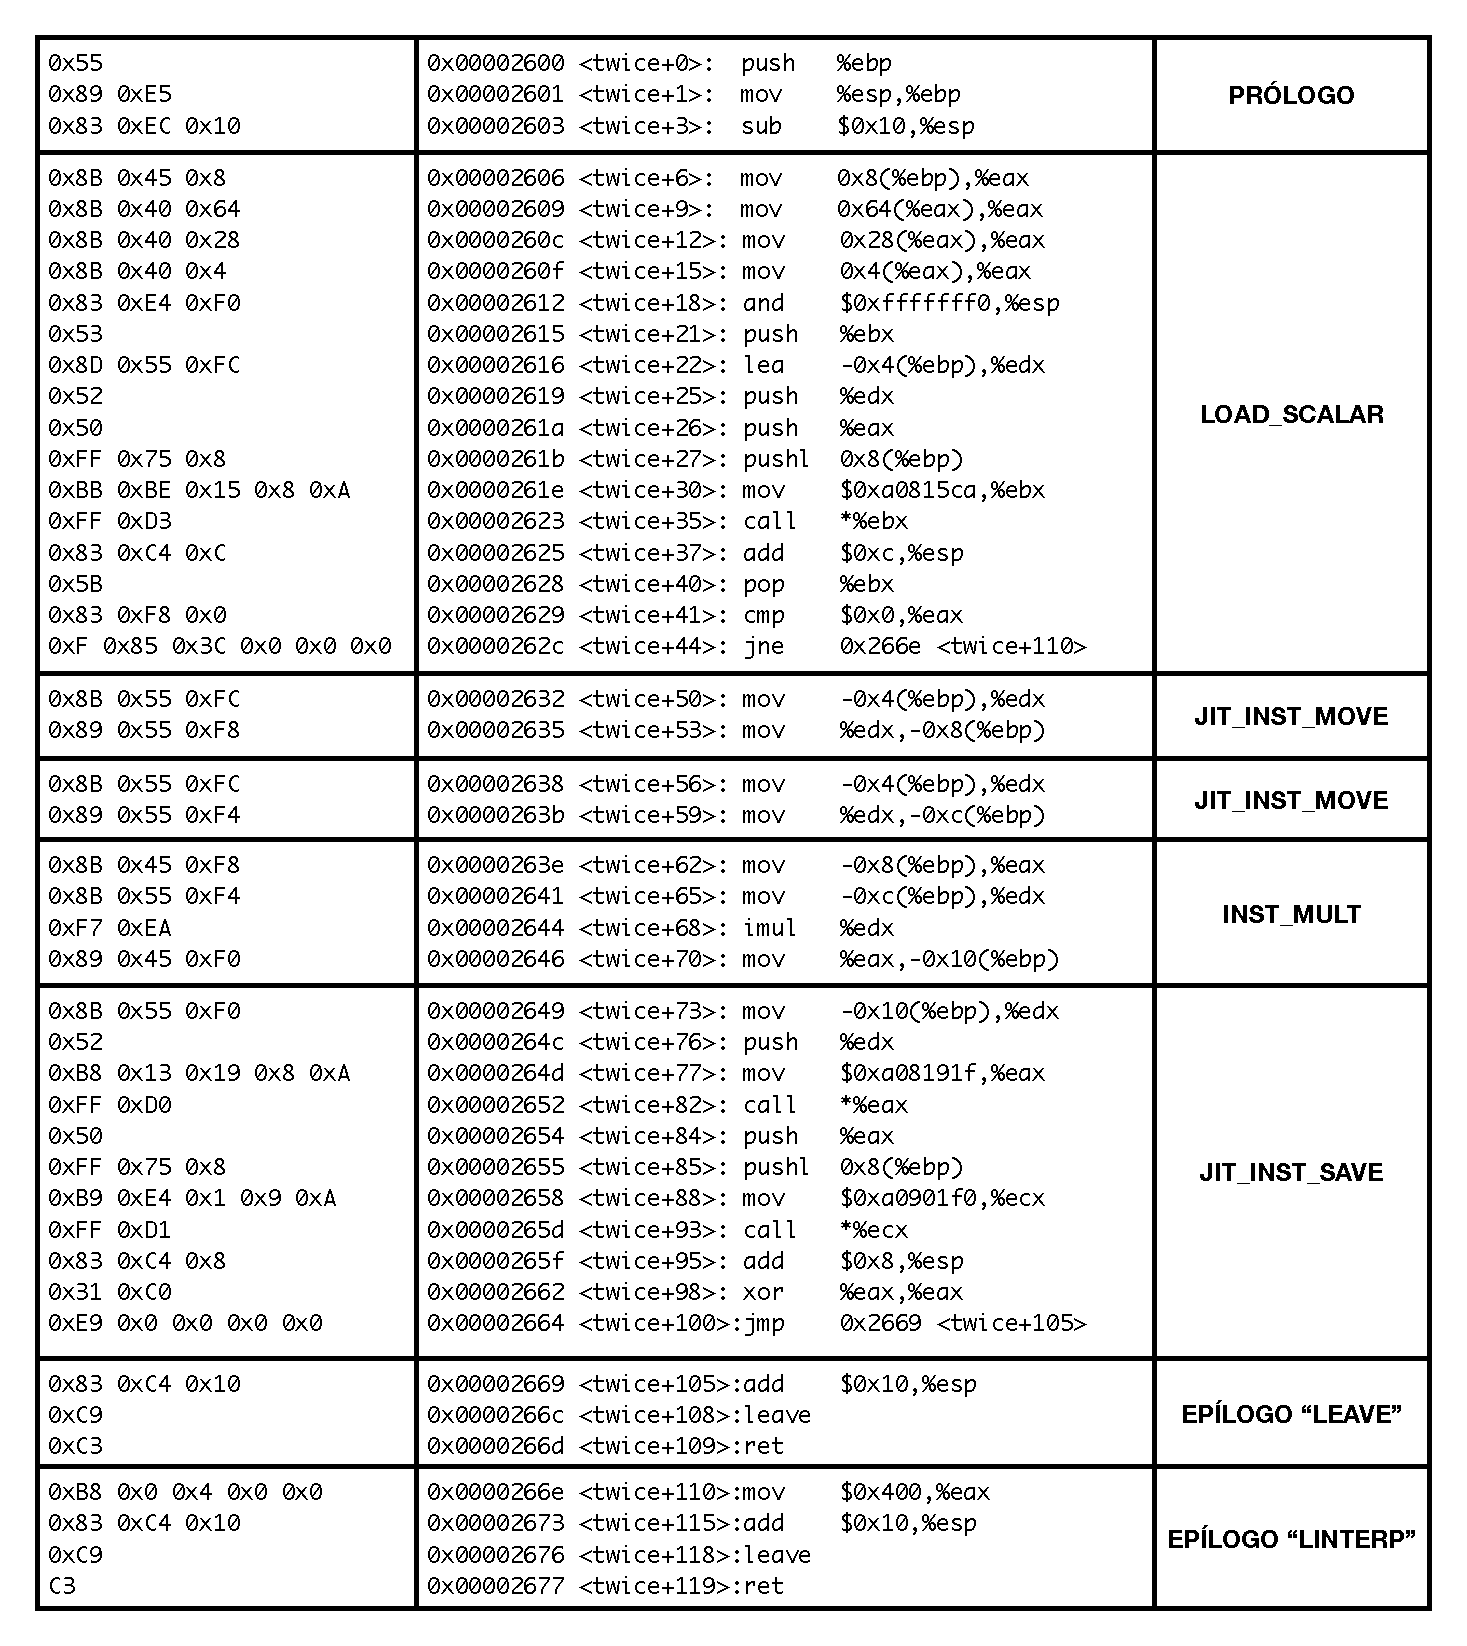
\includegraphics[scale=0.68]{figs/codelongo}
\end{table}

Apesar do procedimento codificado ser bastante simples, é possível
reutilizar código para outras instruções.
 A parte do código que acessa
variáveis locais é reaproveitada pelo código que acessa objetos
literais, com pequenas modificações. A movimentação entre
registradores é utilizada na grande maioria das instruções aceitas, e
com pequenas modificações no código da instrução de multiplicação
consegue-se realizar outras operações aritméticas.

% XXX Talvez colocar alguma coisa assim, melhor explicado.
%Devido a dinamicidade da linguagem \texttt{Tcl}, a coleta de
%tipos realizada em tempo de execução não conseguiu demonstrar
%utilidade na geração de código.
%acabou não demonstrado uso real na geração de código. Seria
%necessário uma forma eficiente para determinação de tipos, mas não
%foi encontrado.

\chapter{Avaliação Experimental}
\label{avaliacao}

\section{Metodologia}
\label{sec:metodologia}

%\begin{itemize}
%\item o que e como avaliar
%\item quais programas serão utilizados na avaliação
%\end{itemize}

% Reordenar frases: A segunda passa a ser a última.
Para avaliar o desempenho do compilador JIT desenvolvido, foi feita uma
análise detalhada com seis \textit{benchmarks} simples. Todos os
testes foram realizados em um computador com processador Intel Core 2
Duo, modelo E4700; memória principal de 2 GiB de 666 MHz, DDR2 DIMM;
\textit{kernel} Linux 2.6.32-25-generic. Foram coletados dados acerca
de: tempo total de execução (\textit{wallclock}),
tempo da compilação JIT, tempo exclusivo de execução de procedimentos
com e sem o JIT desenvolvido.
% XXX Talvez coletar mais usando o PAPI, cache l1 hit/miss
Em todos os casos fez-se uso da ferramenta PAPI \cite{papisite}
 4.1.1 e,
com exceção do \textit{wallclock}, a implementação da \texttt{Tcl} foi
instrumentada para coletar os dados específicos. Foram utilizadas duas
versões da \texttt{Tcl} 8.5.7, a padrão e outra modificada que inclui
o compilador JIT.
% Talvez medir tamanho do código gerado pelo JIT.

\section{Benchmarks}

A implementação atual do compilador cobre apenas um subconjunto
da linguagem \texttt{Tcl}, portanto alguns \textit{benchmarks}
específicos e rudimentares foram criados para possibilitar
uma avaliação inicial. Há uma suíte de testes para a \texttt{Tcl}, a Tclbench
\cite{tclbench-site}, porém somente uma quantidade bastante pequena dos
testes lá existentes podem ser executados com sucesso neste sistema e,
portanto, seu uso não foi considerado.

Em todos os \textit{benchmarks} faz-se uso de um parâmetro $n$ com
significado específico para cada teste. Os \textit{benchmarks}
utilizados foram:
% (códigos ver apêndice
%\ref{apendice-bench}).

\begin{description}
\item[fact] Fatorial iterativo. Calcula $n$ vezes o fatorial dos
  números de 1 a 12
\item[gcd] Máximo divisor comum. Este teste é realizado
  para todos os elementos do produto cartesiano
 $I \times J = \{(i, j) \mid i \in \mathbb{N} \wedge j \in \mathbb{N},
 i \le n \wedge j \le n\}$
\item[gray] Calcula o código gray \cite{graycode} de um número;
  quase um \textit{microbenchmark}. O parâmetro $n$ indica um
  intervalo $[0, n)$ para ter seus respectivos códigos gray gerados.
\item[prime] Verifica se um número é primo ou não. Parâmetro $n$
  define o intervalo ($[0, n]$) de números a serem verificados.
\item[sum$_1$] Somatório de números naturais no intervalo
 $[1, i]$, onde $i$ representa o número da iteração atual no intervalo
 $[1, n]$
\item[sum$_2$] Somatório definido por:
\[ \sum_{i=0}^k a_i\mbox{, onde } a_i = \left\{
    \begin{array}{c l}
      i & \mbox{se } i \mbox{ mod } 4 = 0 \\
      -i & \mbox{se } i \mbox{ mod } 3 = 0 \\
      0
    \end{array}
  \right.
\] com $k$ equivalente a iteração atual no intervalo $[1, n]$
\end{description}


\section{Desempenho}

Para verificar o desempenho a nível macro do compilador JIT,
realizou-se primeiramente a coleta do tempo gasto em execuções
completas. As Figuras
\ref{fig:fact-tempo}, \ref{fig:gcd-tempo}, \ref{fig:gray-tempo},
\ref{fig:prime-tempo}, \ref{fig:sum1-tempo} e \ref{fig:sum2-tempo}
apresentam os dados obtidos para os seis \textit{benchmarks}
distintos. Em todos os casos foram realizadas 100 execuções com tamanho de
$n$ uniformemente espaçado entre os valores mínimo e máximo utilizados.

\begin{figure}[ht!]
  \centering
  \includegraphics[scale=0.70]{figs/fact_tempo}
  \caption{Tempo total de execução para fact \label{fig:fact-tempo}}
\end{figure}
\begin{figure}[ht!]
  \centering
  \includegraphics[scale=0.70]{figs/gcd_tempo}
  \caption{Tempo total de execução para gcd \label{fig:gcd-tempo}}
\end{figure}
\begin{figure}[ht!]
  \centering
  \includegraphics[scale=0.70]{figs/gray_tempo}
  \caption{Tempo total de execução para gray \label{fig:gray-tempo}}
\end{figure}
\begin{figure}[ht!]
  \centering
  \includegraphics[scale=0.70]{figs/prime_tempo}
  \caption{Tempo total de execução para prime \label{fig:prime-tempo}}
\end{figure}
\begin{figure}[ht!]
  \centering
  \includegraphics[scale=0.70]{figs/sum1_tempo}
  \caption{Tempo total de execução para sum$_1$ \label{fig:sum1-tempo}}
\end{figure}
\begin{figure}[ht!]
  \centering
  \includegraphics[scale=0.70]{figs/sum2_tempo}
  \caption{Tempo total de execução para sum$_2$ \label{fig:sum2-tempo}}
\end{figure}

Em grande parde das execuções, a linha que indica o tempo com uso
do compilador JIT permaneceu abaixo da linha do interpretador padrão da
\texttt{Tcl}. Isto era esperado em vista das restrições do sistema
implementado.

Dentre os testes, \textbf{sum$_1$} (Figura
\ref{fig:sum1-tempo}) apresenta a maior
redução (mais de 20 vezes em média). Isto é reflexo do código ali
contido, sendo constituído principalmente de deslocamentos entre
endereços da pilha e soma de inteiros. O gerador de código atual
consegue eliminar boa parde de toda a movimentação de objetos de tipo
\verb!Tcl_Obj!, realizando todas as conversões de \verb!Tcl_Obj! para
inteiro (se possível) num bloco básico especial dedicado para esta
tarefa.
% XXX esse bloco básico especial é aquele gerado na reordenação
% de instruções
Com isso, é possível trabalhar com instruções de máquina que operam
diretamente sobre esses valores inteiros e elimina-se muito do
\textit{overhead} existente na máquina virtual \texttt{Tcl}. O teste
\textbf{sum$_2$} (Figura \ref{fig:sum2-tempo}) também
apresentou um ganho significativo, apesar de fazer uso de divisão por
constante com uso da \verb!IDIV!. Esta é a forma mais simples e geral de
realizar a divisão, mas os compiladores otimizadores a evitam
\cite{opt-invariantintdiv} por consumir muitos ciclos.
%XXX Será que ficou claro por que teve os ganhos ?

Os \texttt{benchmarks} \textbf{fact} (Figura \ref{fig:fact-tempo}),
\textbf{gcd} (Figura \ref{fig:gcd-tempo}) e \textbf{gray} (Figura
\ref{fig:gray-tempo}) não apresentam resultados tão expressivos. No
caso do \textbf{gray}, tem-se que ele é o teste que requer a menor
quantidade de \textit{bytes} para sua codificação e talvez
procedimentos muito pequenos não sejam altamente beneficiados pelo
compilador atual. Os outros dois têm tamanho próximo do
\textbf{sum$_1$}, mas fazem uso de instruções de multiplicação ou
divisão.

Nota-se que \textbf{prime} (Figura \ref{fig:prime-tempo}),
e \textbf{sum$_2$} apresentaram um comportamento
diferenciado nas primeiras execuções. Apesar de $n$ aumentar,
houve um decréscimo de tempo entre a primeira e a segunda
execução nestes casos ao passo em que isto não ocorre quando o código é
interpretado.
Coincidentemente \textbf{prime} e \textbf{sum$_2$} são os que
mais requerem do compilador dinâmico, sendo necessário emitir, na
etapa final, 725 e 609
\textit{bytes}, respectivamente, e, portanto, requerem um tempo maior
na compilação antes da primeira execução nativa. Entretanto, deve-se
notar que os tempos de execução em questão são baixos e que pequenas
modificações no ambiente do sistema operacional podem causar pequenas
flutuações e anomalias nos resultados. Com estes dados, ainda não é
possível concluir que, de fato, o tempo de compilação influenciou
nesse fenômeno observado.

%XXX Quantidade de execuções, nao influencia as curvas ? Talvez
%compilar algo depois de 1 execução nao tenha muita vantagem.

%prime: 768 bytes
%sum2: 633 bytes
%gcd: 401 bytes
%sum1: 363 bytes

%fact: 367 bytes
%gray: 179 bytes

Para facilitar a visualização da diferença de desempenho,
destaca-se a Figura \ref{fig:media-tempo}. O \textit{microbenchmark}
apresenta o menor ganho (cerca de 25\%) mas pode-se verificar que o
tempo gasto pelo laço que
executa o teste domina o tempo total. Somente para executar
\verb!for {set i 0} {$i < $n} {incr i} { .. }!, no maior
teste, gasta-se cerca
de 0,45 segundos, deixando menos de 0,07 segundos para efetivamente
executar o \verb!gray!.

\begin{figure}[ht]
  \centering
  \includegraphics[scale=0.70]{figs/melhoria}
  \caption{Melhoria em relação ao tempo do interpretador padrão (vezes) \label{fig:media-tempo}}
\end{figure}

Apesar de apresentar resultados positivos, os dados exibidos até
agora estão ``contaminados'' com \textit{overhead} herdado da
máquina virtual \texttt{Tcl}. Para deteminar quanto tempo exatamente
é consumido pelo compilador dinâmico, mais dois testes foram
realizados.

Com a Figura \ref{fig:tempo-compilacao} verifica-se que o tempo de
compilação tem influência quase nula no tempo total, custando entre
$49 \times 10^{-6}$ e $79 \times 10^{-6}$ segundos. Também nota-se que
o crescimento do tempo de compilação não acompanha o crescimento dos
\textit{bytes} na mesma proporção.
A linha de tendência 1, para os \textit{bytes}, é
descrita por $y = 10,143x^2 + 31,771x + 168.8$ e apresenta um índice
de correlação com os dados de 0,9379. Enquanto isso, a linha de
tendência 2 é dada por $y = 1,3571x^2 - 3,9x + 52,4$ com índice de
correlação de 0,9876. Onde $1 \le x \le 6$. A tendência é que o tempo
de compilação continue baixo.

\begin{figure}[ht]
  \centering
  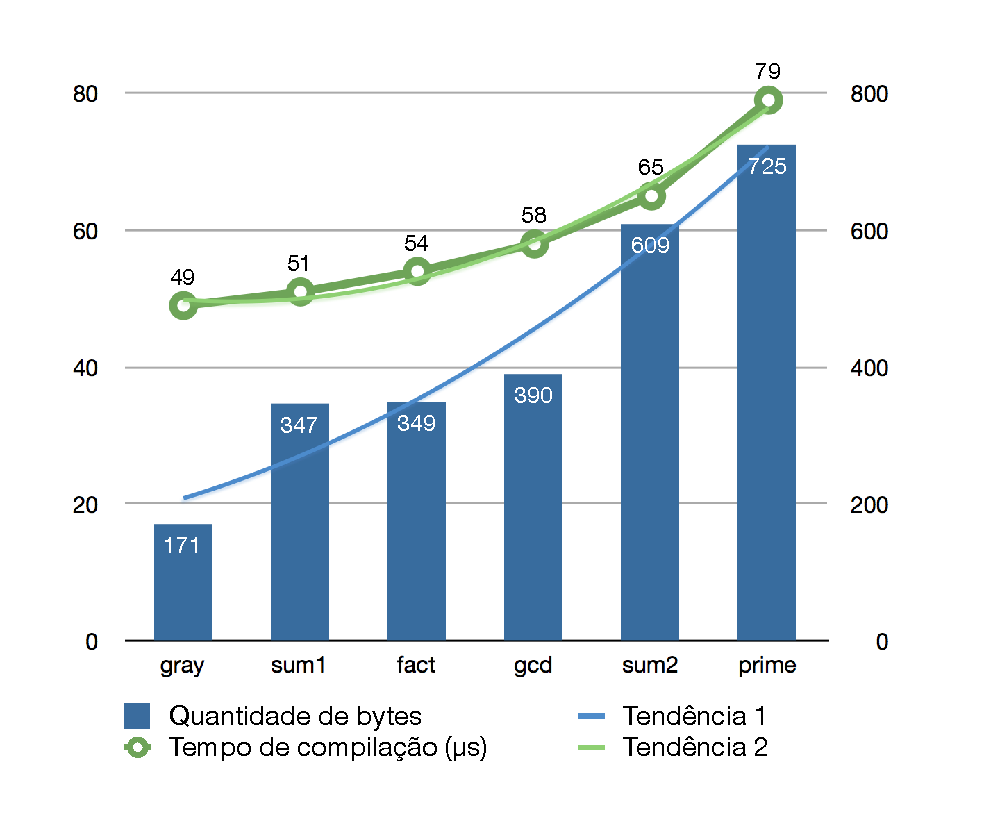
\includegraphics[scale=0.71]{figs/tempo_compilacao}
  \caption{Quantidade de bytes x86 e tempo de compilação \label{fig:tempo-compilacao}}
\end{figure}

A Tabela \ref{tabela-execacc} apresenta os resultados do último teste
desta seção. Para chegar-se a estes dados, utilizou-se dados dos
resultados anteriores para $n$ no maior caso e depois $n$ foi fixado
de acordo com o valor máximo utilizado nos testes específicos de
\textit{wallclock} e, então, foram feitas 10 execuções em cada
situação nova e tomada a média do tempo.

\begin{table}[ht!]
  \caption{Tempo de execução dos \textit{benchmarks} no maior caso\label{tabela-execacc}}
  \centering
  \begin{tabular}{l c c c c c c r}
    \toprule
& \multicolumn{2}{c}{JIT (s)} & \multicolumn{2}{c}{NO JIT (s)} \\
\cmidrule(r){2-3} \cmidrule(r){4-5}
    \textit{Benchmark}  & Total & Exclusivo & Total & Exclusivo & Melhoria (vezes) \\
    \midrule
    fact & 0,14 & 0,04  & 0,30 & 0,19  & 4,75    \\
    gcd & 1,32 & 0,37  & 2,08 & 1,14  & 3,08   \\
    gray & 0,52 & 0,13  & 0,57 & 0,17   & 1,30   \\
    prime & 0,04 & 0,03 & 0,56 & 0,54   & 18,00     \\
    sum$_1$ & 0,46 & 0,44 & 10,60 & 10,22   & 23,22    \\
    sum$_2$ & 0,73 & 0,71 & 11,61 & 10,87   & 15,30     \\
    \bottomrule
  \end{tabular}
\end{table}

% XXX Coletar novamente tempo para prime, sum1 e sum2 nos testes acima.
%XXX Comentar Tabela \ref{tabela-execacc}
A última coluna da Tabela \ref{tabela-execacc} refere-se a melhoria na
nova situação: tempo exclusivo com JIT e sem JIT. Os
\textit{benchmarks} \textbf{fact}, \textbf{gcd} e \textbf{gray} que
tinham tido o menor ganho (Figura \ref{fig:media-tempo}) melhoraram um
pouco se comparados somente seu tempo exclusivo de execução. Isso
indica que o tempo gasto pelo restante do sistema JIT instalado na
\texttt{Tcl} tem impacto menor para menores procedimentos. Entretanto,
também vê-se que o resultado nos demais testes não
foi tão bom quanto antes. No três casos verifica-se que a diferença
entre os tempos das colunas ``Total'' e ``Exclusivo'' para o caso sem
JIT é maior, indicando que o sistema de compilação possa estar
despendendo tempo extra em alguma atividade realizada.

%%% Não consegui fazer dar tempo :/
%\section{Análise Detalhada}

%\begin{itemize}
%\item impaccto do ambiente no hardware
%\item coletar métricas com a ferramenta PAPI
%  (\url{http://icl.cs.utk.edu/papi/})
%\end{itemize}

%%%%%%%%%% XXXX
%* Apesar dos resultados obtidos terem sido tomados a partir de
%exemplos sintéticos, pode-se ter uma visão do que pode-se melhorar na
%implementação do interpretador da \texttt{Tcl}.

\chapter{Conclusões}
\label{conclusao}

%\begin{itemize}
%\item contexto
%\item o que foi feito
%\item resultados obtidos
%\item trabalhos futuros
%\end{itemize}

Um compilador não-otimizador JIT de modo misto para um subconjunto da
linguagem \texttt{Tcl} foi
desenvolvido e validou-se a melhoria de desempenho por meio da
compilação dinâmica. Foi demonstrado um aumento de desempenho de mais
de 29 vezes no melhor caso. Também verificou-se que o tempo
de compilação foi baixo, levando cerca de $79 \times 10^{-6}$
segundos para emitir 725 \textit{bytes}.

Entretanto, mesmo para um pequeno conjunto de
instruções suportadas, a construção do compilador JIT não
foi uma tarefa simples. A geração de código de máquina, em especial
para uma arquitetura CISC, de forma manual é dispendiosa, propensa a
erros e de difícil depuração. Devido a alta
granularidade imposta pela representação intermediária atual,
mostrou-se necessidade de uma quantidade de 120 \textit{bytes}
para a codificação simplificada de um pequeno procedimento em
\texttt{Tcl} que requer apenas 5 quádruplas.
Logo, procedimentos maiores requerem uma quantidade
muito maior de \textit{bytes} e a
verificação da corretude do código gerado é trabalhosa.

Ainda resta descobrir uma forma de coletar tipos de forma eficiente
quando considerada a linguagem \texttt{Tcl}. Mesmo com informações
existentes em tempo de execução, a linguagem não tem um modelo bem
definido de identificação de tipos. Isso é resultado do conceito
fundamental que cerca a linguagem: tudo é \textit{string}. Sem
realizar esta tarefa, a tarefa de
geração de código de forma eficiente parece não ser possível.
O trabalho presente simplifica esta situação, tenta-se trabalhar com
números inteiros mas, nos casos em que não for possível, também
utiliza-se o interpretador.

%XXX Falar que as melhorias encontradas podem estar indicando pontos de
%melhoria no interpretador Tcl

A vantagem de desempenho ao empregar um compilador JIT é
clara. Por esta razão, a técnica tem feito parte das implementações de
máquinas virtuais que demandam alta performance. Entre as linguagens de
programação, \texttt{Java} destaca-se
ao ter recebido suficiente atenção ao ponto de empresas e
pesquisadores desenvolverem diversas JVMs com compiladores
dinâmicos que fazem uso de uma variedade de técnicas.

% Escolhas adequadas para todas as partes de um compilador JIT tornam
% possível o uso de um compilador otimizador em tempo de execução. Esse
% texto teve maior foco nas representações intermediárias utilizadas, ou
% que se pretende utilizar, nesse projeto. Quádruplas para formar blocos
% básicos e permitir a construção do grafo de fluxo de controle (CFG)
% foi mais discutida aqui, mas também foi mencionado a representação SSA
% que inicia-se com a entrada de um CFG. A SSA tem sido aplicada em
% diversos compiladores otimizadores, pois permite aplicar, ao menos,
% as otimizações de movimentação de código, propagação de constante e
% eliminação de redundância parcial de forma eficiente.

% A conversão de \textit{bytecodes} de uma máquina de pilha para uma
% representação na forma de máquina de registradores exige atenção aos
% detalhes da semântica implementada na máquina virtual atual da
% linguagem. Uma vantagem visível é a capacidade de sintetização que
% uma representação baseada em registradores tem sobre uma que faz uso
% de pilha. Entretanto, um número reduzido de quádruplas não indica
% necessariamente menor consumo de memória do que uma quantidade
% superior de \textit{bytecodes}.

% Detalhes relacionados a definição de onde instalar o compilador JIT na
% linguagem alvo e de quando executar a compilação JIT envolvem pelo
% menos um entendimento simplificado do funcionamento da máquina
% virtual. Com a experiência adquirida até o momento, essa etapa aparenta
% ser a mais simples de ser feita.

% A geração de código de máquina, em especial para uma arquitetura CISC,
% de forma manual é dispendiosa e propensa a erros. Apesar da alta
% granularidade imposta pela representação intermediária atual,
% mostrou-se necessidade de 51 bytes para a codificação simplificada de um
% procedimento em \texttt{Tcl} com um único comando
% \verb!incr!. Entretanto, discute-se que, entre essa quantidade total,
% um número significativo de bytes pode ser reaproveitado por muitas das
% outras instruções para acesso a variáveis locais. Além disso, com
% pequenas alterações é possível codificar outras instruções simples, ou
% variações do \verb!incr! que não façam uso de incremento de valor
% absoluto 1, da linguagem \texttt{Tcl}.


% \section{Dificuldades Encontradas}

% A primeira dificuldade encontrada foi em relação a aprendizagem
% (parcial) do funcionamento da linguagem de programação \texttt{Tcl} --
% especificamente a versão 8.5.8 --
% que contém mais de 200 mil linhas de código \texttt{C}. Boa parte
% desse número de linhas não afeta diretamente a construção desse
% compilador, porém uma grande quantidade será ativada
% ao longo da execução do código gerado pelo compilador.

% A linguagem faz uso de contagem de referências para realizar coleta de
% lixo e também compartilha muitos dos valores utilizados. Com isso,
% reutilizar objetos \verb!Tcl_Obj! (atualmente no caso da função
% \verb!JIT_Compile!) que foram construídos em partes distintas não é tão
% simples pois é necessário se ter certeza de que o objeto não será
% desalocado enquanto se está trabalhando com ele e, ao mesmo tempo, não
% se quer deixar objetos com contagem de referência superior a
% necessária. Compartilhar objetos economiza memória mas não simplifica
% o uso de objetos alheios, sendo necessário verificar se um objeto
% específico é compartilhado ou não antes de, dependendo do uso,
% duplicar o mesmo. Não são tarefas tão complexas mas tendem a ser
% pontos de erros obscuros em programas não tão curtos e não tão simples.

% Com o avanço da implementação, descrita nesse relatório, a geração de
% código nativo realizada de forma manual demonstrou-se bastante
% propensa a erros. Detalhes na geração do byte ModR/M causaram muitas
% falhas de segmentação até chegar ao código final correto; saídas
% produzidas pelo compilador gcc, analisada pelas ferramentas \verb!otool! ou
% \verb!objdump!, ajudaram na correção ao longo do processo.

\section{Trabalhos futuros}

O trabalho desenvolvido pode ser considerado como um compilador
\textit{baseline} para um conjunto da \texttt{Tcl}. Desse modo, ainda
falta explorar a utilização de um compilador otimizador.
A conversão de \textit{bytecodes} da máquina de pilha para a
representação na forma de máquina de registradores trouxe as
ineficiências em relação a carregamento e armazenamento de
dados. Logo, este é um primeiro ponto a ser tratado. Além disso, a
alocação de registradores é inexistente e simplesmente atribui-se
posições na pilha para cada registrador virtual. O compilador
otimizador poderia trabalhar sobre estes problemas.

Em relação a representação intermediária, ainda é necessário pelo
menos outra de mais baixo nível. A representação atual está muito
longe do código final, dificultando o processo de alocação de
registradores e seleção de instruções de forma eficiente.
Em um primeiro momento pretendeu-se já fazer uma representação de
baixo nível, mas a conversão de \textit{bytecodes} \texttt{Tcl} para
esta de nível médio demonstrou-se simples e conseguiu-se eliminar
detalhes da máquina de pilha.
Logo, essa nova representação seria mais bem-vinda  se acoplada a
atual.

Aceitando apenas procedimentos folha, um recurso fundamental da
linguagem \texttt{Tcl} fica excluído. Por ser uma linguagem de
comandos, não suportar a realização de chamadas é uma grande
restrição. O trabalho a ser desenvolvido nesta direção precisa se
preocupar com os detalhes de interação entre: \begin{inparaenum}[(1)] \item
  máquina virtual e código nativo; \item código nativo e código
  nativo\end{inparaenum}.


\bibliographystyle{anbt-alfheng}
\bibliography{biblio}

\chapter*{Apêndice A. Código para alocação e ajuste de páginas}
\label{apendiceA}

%XXX
%O código apresentado a seguir ... jit/ em tclsource/generic/, precisa
%modificar o Makefile também em tclsource/unix/ ..., também tem umas
%modificações na própria Tcl que ainda precisam ser incluídas aqui.

\renewcommand\lstlistingname{Código}

\begin{lstlisting}[language=C, caption={Alocação de página(s) para o
    compilador JIT}, frame=tb]
void *
newpage(void *size)
{
    void *page;
#ifdef _WIN32
    page = VirtualAlloc(NULL, *((DWORD *)size),
                        MEM_COMMIT | MEM_RESERVE,
                        PAGE_EXECUTE_READWRITE);
    if (!page) {
        perror("VirtualAlloc");
        exit(1);
    }
#else
    page = mmap(NULL, *((size_t *)size),
                PROT_READ | PROT_WRITE | PROT_EXEC,
                MAP_ANON | MAP_PRIVATE, 0, 0);
    if (page == MAP_FAILED) {
        perror("mmap");
        exit(1);
    }
#endif
    return page;
}
\end{lstlisting}

\begin{lstlisting}[language=C, caption={Tamanho, em bytes, de uma
    página}, frame=tb]
#ifdef _WIN32
DWORD
pagesize(void)
{
    DWORD pagesize;
    SYSTEM_INFO si;
    GetSystemInfo(&si);
    return si.dwPageSize;
}
#else
int pagesize(void)
{
    return getpagesize();
}
#endif
\end{lstlisting}


\begin{lstlisting}[language=C, caption={Remoção da permissão de
    escrita de uma ou mais páginas}, frame=tb]
void
pagenowrite(void *page, size_t len)
{
#ifdef _WIN32
    DWORD oldProtect;
    if (VirtualProtect(page, len, PAGE_EXECUTE_READ,
                       &oldProtect) == 0) {
        perror("VirtualProtect");
        exit(1);
    }
#else
    if (mprotect(page, len, PROT_READ | PROT_EXEC) < 0) {
        perror("mprotect");
        exit(1);
    }
#endif
}
\end{lstlisting}

% \lstset{language=C, frame=tb}

% \lstinputlisting[title=jit/tclJitCodeGen.h]{code/generic/jit/tclJitCodeGen.h}
% \lstinputlisting[title=jit/tclJitCodeGen.c]{code/generic/jit/tclJitCodeGen.c}
% \lstinputlisting[title=jit/tclJitCompile.h]{code/generic/jit/tclJitCompile.h}
% \lstinputlisting[title=jit/tclJitCompile.c]{code/generic/jit/tclJitCompile.c}
% \lstinputlisting[title=jit/tclJitConf.h]{code/generic/jit/tclJitConf.h}
% \lstinputlisting[title=jit/tclJitExec.h]{code/generic/jit/tclJitExec.h}
% \lstinputlisting[title=jit/tclJitInsts.h]{code/generic/jit/tclJitInsts.h}
% \lstinputlisting[title=jit/tclJitOutput.h]{code/generic/jit/tclJitOutput.h}
% \lstinputlisting[title=jit/tclJitOutput.c]{code/generic/jit/tclJitOutput.c}
% \lstinputlisting[title=jit/tclJitTypeCollect.h]{code/generic/jit/tclJitTypeCollect.h}
% \lstinputlisting[title=jit/tclJitTypeCollect.c]{code/generic/jit/tclJitTypeCollect.c}

% \lstinputlisting[title=jit/arch/arch.h]{code/generic/jit/arch/arch.h}
% \lstinputlisting[title=jit/arch/x86/mcode.h]{code/generic/jit/arch/x86/mcode.h}
% \lstinputlisting[title=jit/arch/x86/mcode.c]{code/generic/jit/arch/x86/mcode.c}





\pagebreak


~~\\

\vspace{18cm}

\begin{center}

\textbf{Universidade Estadual de Maringá}

\textbf{Departamento de Informática}

\textbf{Av. Colombo 5790, Maringá - PR, CEP 87020-900}

\textbf{Tel: (44) 3261-4324 Fax: (44) 3263-5874}

\textbf{www.din.uem.br}

\end{center}

\pagebreak



\end{document}
